\part{序論}

\vspace{0.7cm}
\begin{quote}
「チャイナタウンで道に迷わず歩くことさえ十分に難しいというのに，

宇宙を『知ろう』とする人たちには驚かされる」

{\it Woody Allen}
\end{quote}


\vspace{0.2cm}


 \begin{figure}[h!]
    \centering
        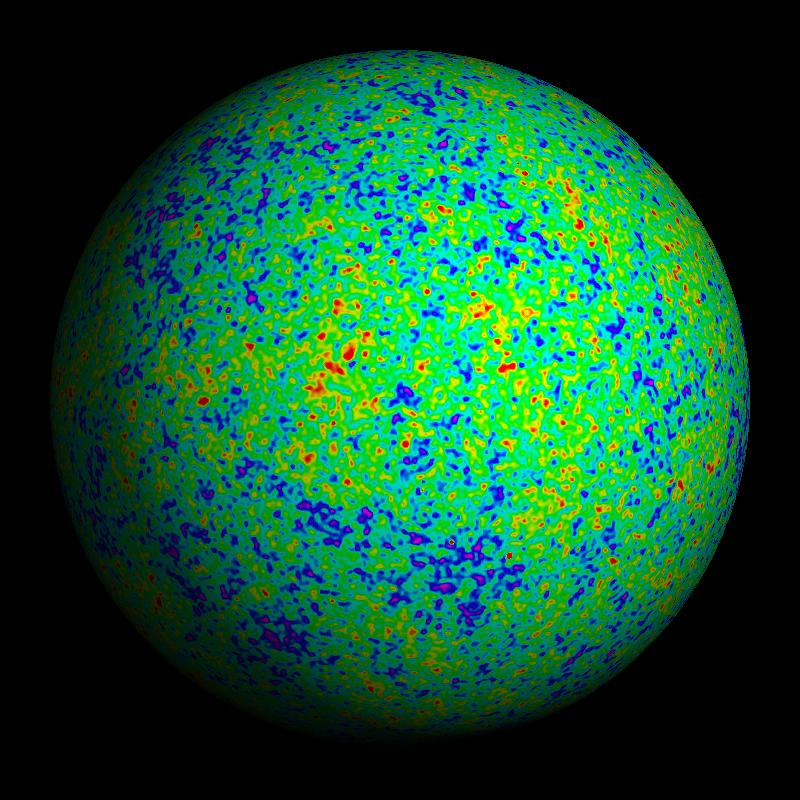
\includegraphics[width=.45\textwidth]{./CMB.jpg}
\caption{宇宙マイクロ波背景放射（CMB）の揺らぎ．何がこれを生み出したのだろうか．}
    \label{fig:CMB1}
\end{figure}
 

%\sectionlink{Introduction}
\sectionlink{構造の微視的起源}

\subsectionlink{TASI 2009：{\sl 大きなものと小さなものの物理}}

%{\tt more}

宇宙マイクロ波背景放射（CMB）の温度揺らぎ（図~\ref{fig:CMB1}参照）は，驚くべき物語を伝えている．現在ではウィルキンソン・マイクロ波異方性探査機（WMAP）などの実験によってほぼ日常的に測定されるようになったマイクロ波の天空の温度変動は，原始宇宙の密度に微小な揺らぎがあったことを物語っている．
これらの揺らぎは重力不安定性によって成長し，現在の宇宙で観測される大規模構造（LSS）になった．%of the late-time universe.
ビッグバンの熱的な残光の観測を，数十億年後の構造形成に結び付けることに成功した私たちは，さらに大胆な問いへと向かう．CMBの揺らぎの根本的な微視的起源は何だろうか．
この問いに答えることは，宇宙のあらゆる構造の物理的起源を根本から理解することにほかならない．

本講義では，宇宙の{\it インフレーション}期が，この構造の形成と進化の描像に不可欠な一部をなしていたという，現在最も有力な作業仮説を解説する．
インフレーション\cite{Guth:1980zm, Linde:1981mu, Albrecht:1982wi}とは極初期宇宙における指数関数的膨張の時期であり，ビッグバン特異点の約$10^{-34}$秒後に起こったと考えられている．
驚くべきことに，インフレーションは，宇宙の大域的な一様性と，私たちの銀河のような構造が形成される種となった小さな揺らぎの，両方を生み出したと考えられている．

この連続講義の中心となるのは，インフレーションが微視的な量子揺らぎを宇宙のエネルギー密度の巨視的な揺らぎへと変換した物理的機構を，詳しく説明することである．
この意味でインフレーションは，{\sl TASI 2009}の主題である「大きなものと小さなものの物理」のつながりを示す，最も劇的な例を与える．
インフレーションが生み出す揺らぎのスペクトルの統計的性質とスケール依存性を，具体的に計算する．この結果は，宇宙の構造形成を扱うすべての研究への入力となり，現代理論宇宙論の大きな成果の一つである．



\subsectionlink{宇宙の構造と進化}

宇宙の膨張には否定しようのない証拠がある．遠方の銀河からの光は，スペクトルの赤い側へ系統的にずれている\cite{Hubble}．軽元素（H，He，Li）の観測存在量は，ビッグバン元素合成（BBN）の予言と一致する\cite{abc}．そして，CMBについて説得力のある唯一の説明は，それが高温の初期宇宙から残った放射だというものである\cite{DickeCMB}．
 
 \begin{figure}[h!]
    \centering
        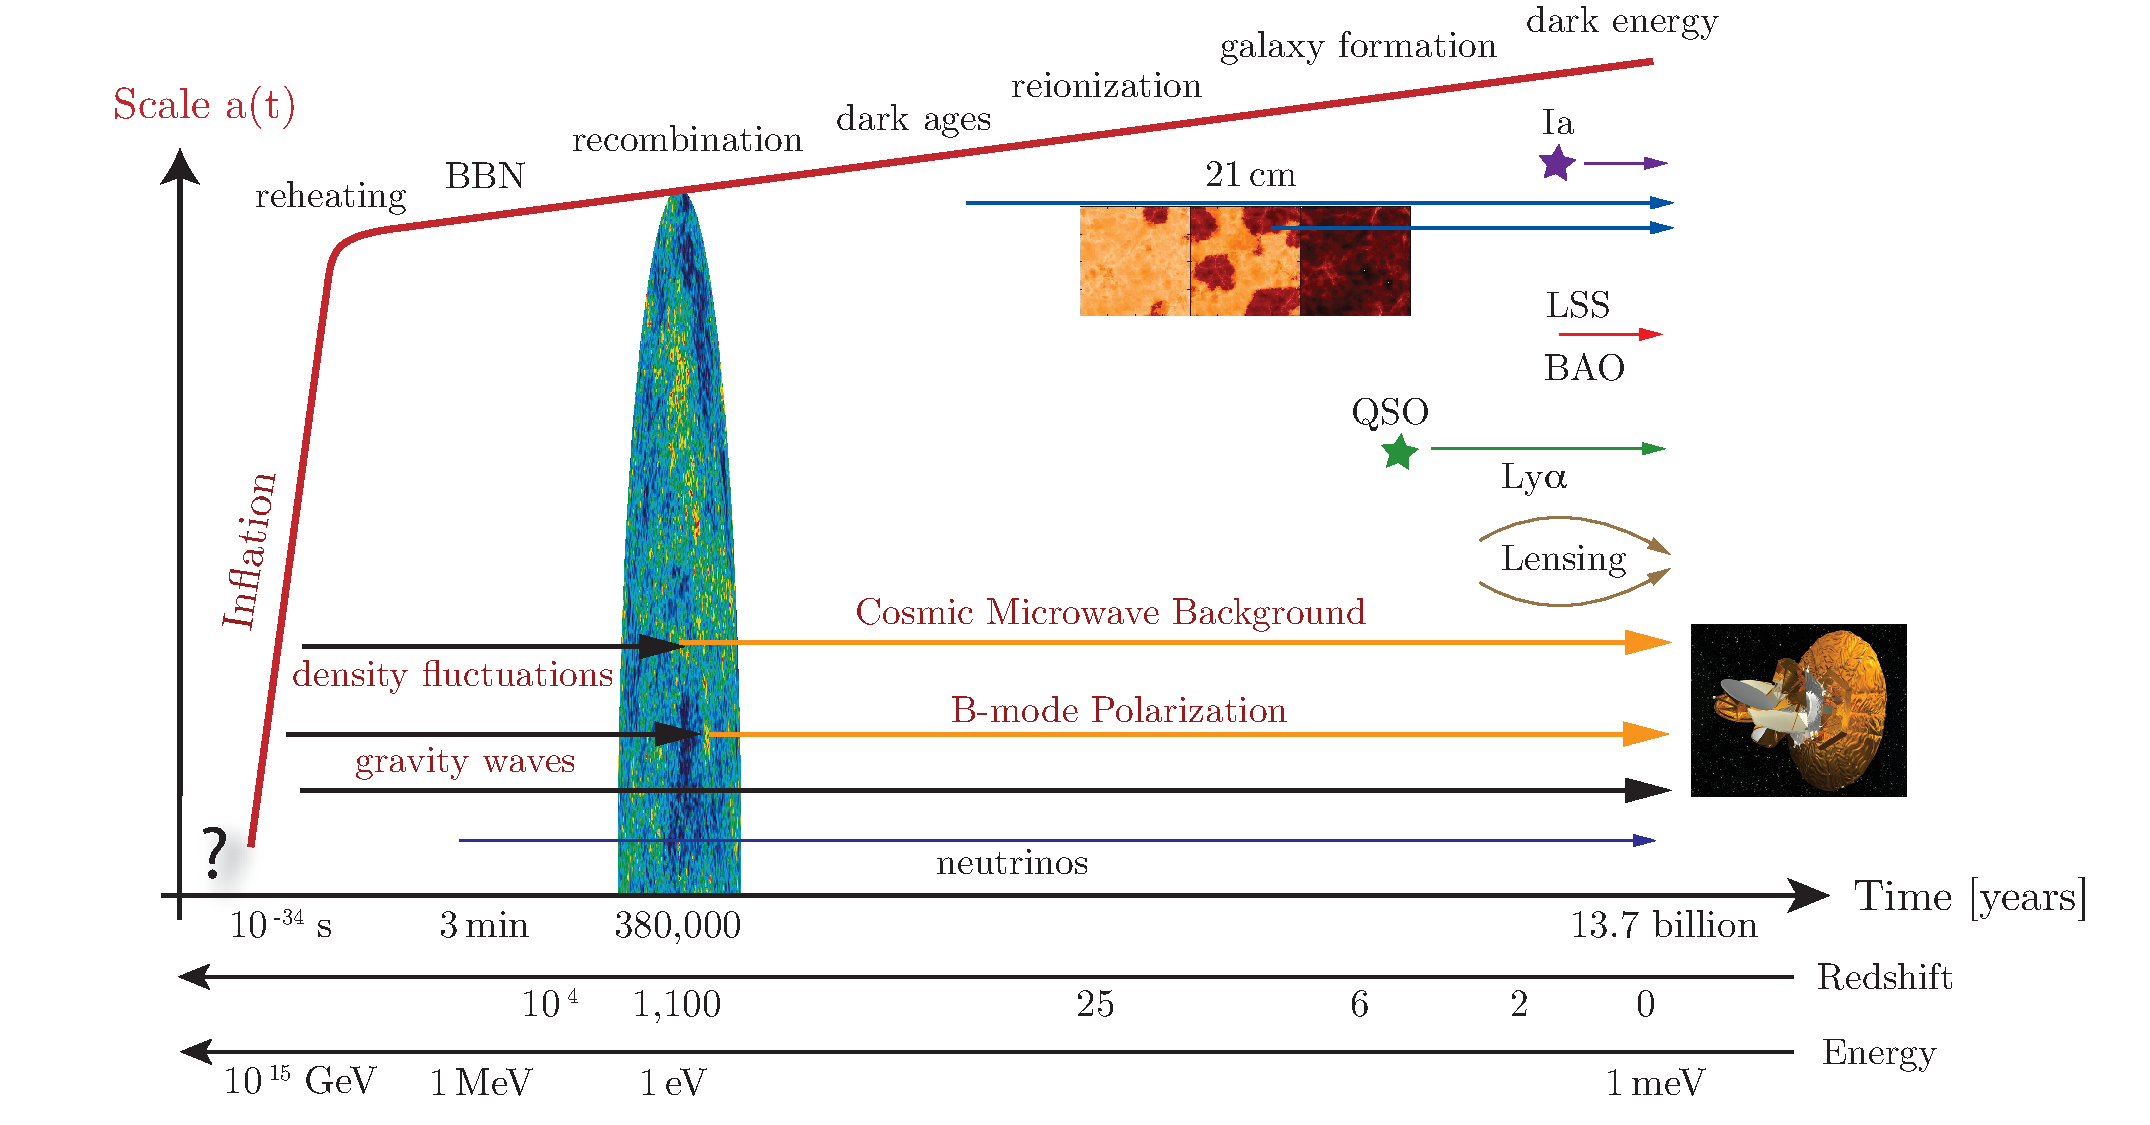
\includegraphics[width=1.0\textwidth]{./timeline}
\caption{宇宙の歴史．この模式図には，宇宙史の主要な出来事と，それに対応する時間およびエネルギースケールを示す．また，宇宙の構造と進化について情報を与える，いくつかの宇宙論的観測手段も示す．%\newline
{\small {\it 略語}：BBN（ビッグバン元素合成），LSS（大規模構造），BAO（バリオン音響振動），QSO（準恒星状天体＝クエーサー），Ly$\alpha$（ライマン・アルファ），CMB（宇宙マイクロ波背景放射），Ia（Ia型超新星），21cm（水素の21cm遷移）．}}
    \label{fig:timeline}
\end{figure}
 
膨張宇宙における熱力学と素粒子物理学を特徴付ける原理は二つある．
{\sl i)} 相互作用率が膨張率を下回ると，粒子間の相互作用が凍結すること，
{\sl ii)} 物理法則における破れた対称性は，高エネルギーで回復しうることである．
表~\ref{tab:timeline}に，宇宙の熱史と，対称性の破れに関係するさまざまな相転移を示す．
以下では，私たちの宇宙の進化を画するこれらの出来事を，定性的に簡潔に概観する．
この宇宙史のどの側面が確立された物理学に基づき，どの側面により推測的な考えが必要なのかを強調する．
% to celebrate the achievements of physics and cosmology in the past century.
%We will emphasize which aspects we consider certain and which are still more speculative.

\begin{table}[h!]
\caption{宇宙史の主要な出来事．}
\label{tab:timeline}
\begin{center}
\begin{tabular}{l | r | r | r}
 & {\small 時間} & {\small エネルギー} & \\
 \hline 
 \hline
 {\small プランク期？} & {\small $< 10^{-43}$ s} & {\small $10^{18}$ GeV} &\\
 {\small 弦スケール？} & {\small $\gtrsim 10^{-43}$ s} & {\small $\lesssim 10^{18}$ GeV} & \\
{\small 大統一？} & {\small $\sim 10^{-36}$ s} & {\small $10^{15}$ GeV} & \\
{\small インフレーション？} & {\small $\gtrsim 10^{-34}$ s} & {\small $\lesssim 10^{15}$ GeV} &\\
{\small 超対称性の破れ？} & {\small $< 10^{-10}$ s} & {\small $> 1$ TeV} &\\
{\small バリオン数生成？} & {\small $< 10^{-10}$ s} & {\small $> 1$ TeV} &\\
\hline
\hline
{\small 電弱統一} & {\small $10^{-10}$ s} & {\small 1 TeV} &\\
{\small クォーク・ハドロン転移} & {\small $10^{-4}$ s} & {\small $10^2$ MeV} &\\
{\small 核子の凍結} & {\small 0.01 s} & {\small 10 MeV} &\\
{\small ニュートリノの脱結合} & {\small 1 s} & {\small 1 MeV} &\\
{\small BBN} & {\small 3 min} & {\small 0.1 MeV} &\\
\hline 
\hline
& & & {\small 赤方偏移} \\
\hline 
\hline
{\small 物質・放射等価} & {\small $10^4$ 年} & {\small 1 eV} & {\small $10^4$}\\
{\small 再結合} & {\small $10^5$ 年} & {\small 0.1 eV} & {\small 1,100}\\
{\small 暗黒時代} & {\small $10^5 - 10^8$ 年} & & {\small $> 25$} \\
{\small 再電離} & {\small $10^8$ 年} & & {\small $25 - 6$}\\
{\small 銀河形成} & {\small $\sim 6 \times 10^8$ 年} & & {\small $\sim 10$} \\
{\small ダークエネルギー} & {\small $\sim 10^9$ 年} & & {\small $\sim 2$} \\
{\small 太陽系} & {\small $8 \times 10^9$ 年} & & {\small 0.5} \\
{\small アルベルト・アインシュタイン誕生} & {\small $14 \times 10^{9}$ 年} & {\small 1 meV} & {\small 0} \\
\hline
\end{tabular}
  \end{center}
\end{table}

$10^{-10}$秒から現在までの宇宙史は，よく理解され，実験的に検証された素粒子物理学，原子核・原子物理学，および重力の法則に基づいている．
したがって，その間に宇宙を形作った出来事について，ある程度の確信を持つことには根拠がある．
% (see Figure~\ref{fig:timeline} and Table~\ref{tab:timeline}).

電弱相転移の時刻（$10^{-10}$\,s），$100$ GeVの宇宙に入ってみよう．
$100$ GeVより上では電弱対称性が回復し，$Z$および$W^\pm$ボソンは質量を持たない．
相互作用は，クォークとレプトンを熱平衡に保つのに十分強い．
$100$ GeVより下では，電磁力と弱い力の間の対称性が破れ，$Z$および$W^\pm$ボソンは質量を獲得する．そして宇宙の温度の低下とともに，弱い相互作用の断面積が減少する．
その結果，$1$ MeVでニュートリノは他の物質から脱結合する．
その直後の$1$秒には，温度が電子の静止質量を下回り，電子と陽電子が効率よく対消滅する．初期に存在した10億分の1の物質・反物質非対称性だけが生き残る．
こうして生じた光子・バリオン流体は平衡状態にある．
$0.1$ MeV付近で強い相互作用が重要になり，ビッグバン元素合成（$\sim 200$\,s）の間に陽子と中性子が結合して軽元素（H，He，Li）を形成する．H，He，Liの存在量の予言が成功したことは，ビッグバン理論の最も目覚ましい帰結の一つである．
物質密度と放射密度は$1$ eV（$10^{11}$\,s）付近で等しくなる．
プラズマ中では，荷電した物質粒子と光子が強く結合しており，密度の揺らぎは宇宙の「音波」として伝播する．
$0.1$ eV付近（38万年）で陽子と電子が結合して，中性の水素原子となる．
光子は脱結合し，自由に伝播する宇宙マイクロ波背景放射を形成する．
137億年後，これらの光子は宇宙の最も古いスナップショットを私たちに届ける．
CMB温度の異方性は，原始物質密度の揺らぎの証拠を与える．
% of the early universe.

これらの小さな密度摂動$\rho({\bf x}, t) = \bar \rho(t) [1+ \delta({\bf x}, t)]$は，重力不安定性によって成長し，後期宇宙で観測される大規模構造を形成する．
背景の圧力と普遍的な重力の引力との競合が，構造の成長の詳細を決める．
放射優勢期の成長は遅く，$\delta \sim \ln a$である（ここで$a(t)$は空間の膨張を記述するスケール因子）．物質が背景密度を支配するようになると（圧力がゼロに下がり），集積はより効率的になり，$\delta \sim a$となる．まず小さなスケールが非線形化し，$\delta \gtrsim 1$となって，全体の膨張から切り離された重力的に束縛された天体を形成する．
これによって，まず小さなスケールの構造（恒星や銀河など）が形成され，次いで合体してより大きな構造（銀河団や超銀河団）になるという，階層的構造形成の描像が得られる．
赤方偏移$z \sim 25$（$1+z = a^{-1}$）付近で，最初の恒星からの高エネルギー光子が銀河間物質中の水素を電離し始める．この「再電離」の過程は$z \approx 6$で完了する．
一方，最も大質量の恒星は核燃料を使い果たし，「超新星」として爆発する．
これらの爆発の中で，生命の形成に必要な重元素（C，O，\dots）が作られる．これが「私たちは皆，星屑でできている」という言葉の由来である．
$z \approx 1$では，負の圧力を持つ「ダークエネルギー」が宇宙を支配するようになる．
背景時空の膨張は加速し，構造の成長は止まって，$\delta \sim$一定となる．


\subsectionlink{最初の$10^{-10}$秒}

$10^{-10}$秒（1~TeV）から現在までの宇宙史は，観測事実と，素粒子物理学の標準模型，一般相対性理論，流体力学などの検証済みの物理理論に基づく．例えば，高エネルギー物理学の基本法則は，現在の粒子加速器が到達するエネルギー（$\sim 1$~TeV）まで十分に確立されている．
$10^{-10}$秒より前には宇宙のエネルギーが1~TeVを超え，実験が直接導いてくれるという安心感を失う．
したがって，この時代の物理学は，魅力的であるのと同じくらい推測的でもある．

CMB温度に見られる揺らぎを説明するには，種となる原始揺らぎを入力しなければならない．
本講義では，これらの原始揺らぎが極初期宇宙（$\sim 10^{-34}$秒）のインフレーション期に生成されたという仮説を説明する．
エネルギー密度の微視的な量子揺らぎが，インフレーションによる膨張によって，その時点の物理的な地平線よりも大きな巨視的スケールへ引き伸ばされる様子を説明する．
摂動が地平線の外に出ると，因果的な物理過程はそれに影響を与えられなくなる．振幅が一定のまま凍結され，その後の通常の（加速しない）ビッグバン膨張の間に，地平線へ再び入るまでその状態が続く．宇宙の構造に対応する揺らぎは，CMB光子が脱結合する少し前，宇宙年齢が約10万年のときに地平線へ再突入する．
地平線の内部では因果的な物理過程が摂動の振幅に影響を与えることができ，実際にそれがCMBの音響ピーク構造や，高密度の揺らぎが銀河・銀河団へと崩壊する過程をもたらす．
地平線への再突入後の摂動の進化は理解されており，計算することもできるため，後期のCMBやLSSの観測から，入力となった原始スペクトルを推定できる．
このスペクトルがインフレーションによって生成されたと仮定すると，それは宇宙年齢が$10^{-34}$秒であったときの物理的状況を観測的に探る手段となる．
宇宙論を用いて最高エネルギーの物理を探る，この魅力的な可能性が本講義の主題である．

\sectionlink{講義の構成}

{第1講}では，インフレーションの{\it 古典的}な背景力学を導入する．インフレーションが地平線問題と平坦性問題をどのように解決するかを説明する．スローロール条件と再加熱を論じ，インフレーションによる膨張の物理的起源を考察する．
{第2講}では，インフレーション中の{\it 量子}揺らぎが，大規模構造の形成の種となる仕組みを説明する．スカラー摂動とテンソル摂動$\R$および$h_{ij}$のインフレーションによるパワースペクトルを，詳細に導出する．
{第3講}では，第2講の結果を，宇宙マイクロ波背景放射と銀河分布の観測に結び付ける．つまり，天空で$P_\R(k)$と$P_h(k)$をどのように測定するかを説明する！ 現在の観測的制限を述べ，将来のインフレーションの検証を強調する．
{第4講}では，原始揺らぎの非ガウス性の研究における主要な結果を示す．
非ガウス相関から，インフレーションの作用に関する重要な情報がどのように得られるかを説明する．
{第5講}では，現在の研究の最前線にある発展的な話題，すなわち弦理論におけるインフレーションを扱う．
この主題の主要な難問を説明し，最近の進展をまとめる．
%primordial non-Gaussianity.

\vskip 5pt
各講義を自己完結的にするため，それぞれの中心部分に先立つ短い{\sl 復習}の節で，必要な背景知識を示す．
各講義の最後には，最も重要な結果の{\sl まとめ}を置く．
本文中の随所に現れる問題や演習と，講義の末尾に独立した{\sl 問題集}として付した長めの問題は，各講義の重要な一部である．
演習は，講義の内容を補完したり，計算の細部を補ったりするよう，注意深く選んである．

\vskip 5pt
いくつかの付録には，宇宙論的摂動論の標準的な結果と，インフレーション中の摂動計算の詳細をまとめた．これらの付録が，読者にとって有用な参照資料となることを願っている．
%In fact, in recent research projects I frequently found myself consulting these appendices, so I hope that they can be equally useful for others.

\newpage
\subsubsection*{記法}

本講義では，記法に一貫性と整合性を持たせるよう努めた．

全編を通じて，天与の自然単位系を用いる．
\beq
c = \hbar  \equiv 1\, . \nonumber
\eeq
換算プランク質量を次のように定義し，
\beq
M_{\rm pl} = (8 \pi G)^{-1/2}\, , \nonumber
\eeq
しばしばその値を1と置く．
計量の符号は$(-+++)$とする．
ギリシャ文字の添字は$\mu, \nu =0,1,2,3$の値を取り，ラテン文字の添字は$i,j=1,2,3$を表す．
フーリエ変換の規約は
\beq
\R_{\bf k} = \int \d^3 {\bf x}\, \R({\bf x}) e^{-i {\bf k} \cdot {\bf x}}\, , \nonumber
\eeq
とし，したがってパワースペクトルは
\beq
\langle \R_{\bf k} \R_{{\bf k}'} \rangle = (2\pi)^3 \delta({\bf k}+ {\bf k}') P_\R(k) \, , \qquad \Delta_\R^2(k) \equiv \frac{k^3}{2\pi^2} P_\R(k)\, . \nonumber
\eeq
である．共形時間には文字$\tau$を用いる（天体物理学で光学的厚さを表すパラメータと混同しないよう注意されたい）．文字$\eta$は第2スローロール・パラメータのために取っておく．物理的時間に関する微分は上付きのドットで表し，共形時間に関する微分はプライムで表す．
偏微分はコンマ，共変微分はセミコロンで表す．

\subsubsection*{謝辞}

素粒子物理学の理論高等研究所（{\sl TASI}）で本講義を行う機会を与えてくださったScott DodelsonとCsaba Csakiに，深く感謝する．

この数年間，師であるLiam McAllister，Paul Steinhardt，Matias Zaldarriagaと，共同研究者のIgor Klebanov，Anatoly Dymarsky，Shamit Kachru，Hiranya Peiris，Alberto Nicolis，Asantha Coorayから，多くのことを学んだ．
彼らが洞察を惜しみなく分かち合ってくれたことに感謝する．
{\sl CMBPol}インフレーション作業部会\cite{WhitePaper}のメンバーからの助言にも，大いに感謝している．
本講義で扱う多くの話題に関する彼らの専門的な意見は，私にとって極めて貴重であった．
Richard Easther，Eva Silverstein，Eiichiro Komatsu，Mark Jackson，Licia Verde，David Wands，Paolo Creminelli，Leonardo Senatore，Andrei Linde，Sarah Shanderaとの議論からも，多くのことを学んだ．

この講義録の執筆中に温かく迎えてくださったAspen Center for Physics，ボストンのTrident Cafe，ケンブリッジのDado Teaに感謝する．

最後に，質問によって私に挑み，この講義録の草稿に意見を寄せてくれた{\sl TASI 2009}の学生たちに感謝したい．
\newpage
\part{第1講：インフレーションの{\sl 古典的}力学}

\vspace{0.5cm}
 \hrule \vspace{0.3cm}
\begin{quote}
{\bf 要旨}

\noindent
本講義の目的は，インフレーション宇宙論の古典的力学を第一原理から導入することである．
基本的なFRW宇宙論を簡単に復習した後，通常のビッグバン理論が初期条件問題を生じることを示す．すなわち，私たちの知る宇宙は，極めて特殊で微調整された初期条件からしか生まれない．次に，インフレーション（初期の加速膨張期）がこの初期条件問題をどのように解決し，一般的な初期条件から私たちの宇宙が生じることを可能にするかを説明する．
インフレーションに必要な条件を述べ，インフレーションが時空の因果構造をどのように変えて，ビッグバンの謎を解くかを説明する．
最後に，インフレーションによる膨張の物理的起源を論じて本講義を締めくくる．
%We describe single-field slow-roll inflation, reheating, the UV sensitivity of models of inflation and inflation in string theory.
\end{quote}
\vspace{0.1cm}  \hrule
 \vspace{0.5cm}
 
 
%\sectionlink{Cosmological Preliminaries}
%\sectionlink{FRW Cosmology}
\sectionlink{{\sl 復習}：一様な宇宙}
\label{sec:FRW}

準備として，一様な宇宙の基本的な性質を復習する．
この内容は{\sl TASI 2009}におけるTurner教授の講義で扱われ，また宇宙論のどの教科書にも含まれているので（例えば\cite{Dodelson, Mukhanov, WeinbergCosmology}），ここでは簡潔に述べ，多くの概念は読者向けの演習を通じて思い出してもらうことにする．
当然ながら，インフレーションの研究に最も関係の深い事項に焦点を当てる．

\subsectionlink{FRW時空}

宇宙論は，最大のスケールにおける宇宙の構造と進化を記述する．大きなスケールで{\it 一様性}と{\it 等方性}\footnote{{\it 一様な}空間とは，並進不変，すなわちどの点でも同じである空間のことである．{\it 等方的な}空間とは，回転不変，すなわちどの方向でも同じである空間のことである．あらゆる点で等方的な空間は必ず一様であるが，逆は成り立たない．例えば，一様な電場のある空間は並進不変だが，回転不変ではない．}を仮定すると，宇宙の時空を表すフリードマン・ロバートソン・ウォーカー（FRW）計量に導かれる（{\bf 問題~\ref{pro:FRW}}参照）．
\beq
\label{equ:FRW}
\fbox{$\displaystyle
\d s^2 = - \d t^2 + a^2(t)  \left(\frac{\d r^2}{1-k r^2} + r^2 (\d \theta^2 + \sin^2 \theta \d \phi^2) \right) $}\, .
\eeq
ここでスケール因子$a(t)$は，異なる時刻における空間的超曲面$\Sigma$の相対的な大きさを特徴付ける．曲率パラメータ$k$は，$\Sigma$が正の曲率を持つ場合に$+1$，$\Sigma$が平坦な場合に$0$，$\Sigma$が負の曲率を持つ場合に$-1$である．
式~(\ref{equ:FRW})は共動座標を用いている．宇宙は$a(t)$の増加とともに膨張するが，銀河や観測者は，それらに力が働かない限り，すなわち固有運動がない限り，
%\footnote{This statement only applies to the Hubble flow and ignores the peculiar velocities of galaxies ${\bf v}_{\rm pec} = (\dot r, \dot \theta, \dot \phi)$.} 
座標$r$，$\theta$，$\phi$を一定に保つ．
対応する物理的距離はスケール因子を掛けて$R=a(t) r$と求められ，固有速度がゼロの天体であっても時間に依存する．
座標変換によって計量(\ref{equ:FRW})は次のように書ける．
\beq
\label{equ:FRW2}
\fbox{$\displaystyle
\d s^2 = - \d t^2 + a^2(t)  \left(\d \chi^2 + \Phi_k(\chi^2) (\d \theta^2 + \sin^2 \theta \d \phi^2) \right) $}\, ,
\eeq
ここで，
\beq
r^2 = \Phi_k(\chi^2) \equiv  \left\{
\begin{array}{c} \sinh^2 \chi \\ \chi^2 \\ \sin^2 \chi \\
\end{array} \right. \quad \begin{array}{l} k=-1 \\ k=0 \\ k=+1 \end{array}\, .
\eeq
%Here, $r$ and $\chi$ are
%{\it comoving coordinates}. They are related to physical coordinates by the scale factor.
FRWの仮定のもとで，一様な宇宙の進化は一つの関数$a(t)$に帰着する．
その形は，アインシュタイン方程式を通じて宇宙の物質内容によって決まる（\S\ref{sec:EinsteinEqns}参照）．
FRW時空を特徴付ける重要な量が，次の膨張率である．
\beq
\fbox{$\displaystyle
H \equiv \frac{\dot a }{a} $}\, .
\eeq
{\it ハッブル・パラメータ}$H$は時間の逆数の単位を持ち，膨張する宇宙では正（収縮する宇宙では負）である．
これはFRW時空の基本的なスケールを定める．すなわち，一様な宇宙の特徴的な時間スケールはハッブル時間$t\sim H^{-1}$であり，特徴的な長さスケールはハッブル長$d \sim H^{-1}$である（$c=1$の単位系）．ハッブル・スケールは宇宙年齢のスケールを定め，ハッブル長は観測可能な宇宙の大きさを定める．


\subsectionlink{運動学：共形時間と地平線}

宇宙の平均的な時空の計量を定義したので，光や物質粒子の伝播の運動学的性質を調べることができる．

%\vskip 6pt
%\noindent
\subsubsection*{共形時間とヌル測地線}

宇宙の因果構造は，FRW時空(\ref{equ:FRW})における光の伝播によって決まる．質量のない光子は，$\d s^2 = 0$を満たすヌル測地線に沿って進む．これらの光子の軌跡は，次のように共形時間\footnote{共形時間は，宇宙の膨張とともに進み方が遅くなる「時計」と解釈できる．}を定義すると，最も容易に調べられる．
\beq
\fbox{$\displaystyle
\tau = \int \frac{\d t}{a(t)} $}\, ,
\eeq
このときFRW計量は
\beq
\d s^2 =a(\tau)^2 \left[- \d \tau^2 +  \left(\d \chi^2 + \Phi_k(\chi^2) (\d \theta^2 + \sin^2 \theta \d \phi^2) \right) \right] \, .
\eeq
となる．等方的な宇宙では，次の2次元の線素で決まる，光の動径方向の伝播を考えればよい．
\beq
\d s^2 = a(\tau)^2 \left[ - \d \tau^2 + \d \chi^2\right]\, .
\eeq
計量は，静的なミンコフスキー計量に，時間依存する共形因子$a(\tau)$を掛けた形に分解された．
したがって共形時間で表すと，FRW時空における光の動径方向のヌル測地線は，次を満たす．
\beq
\chi(\tau) = \pm \tau\, +\, {\rm const.}\, ,
\eeq
すなわち，$\tau$--$\chi$平面上で角度$\pm 45^\circ$の直線に対応する（図~\ref{fig:lightcone}参照）．
光の伝播を調べるのに物理的時間$t$を使っていたなら，曲がった時空における光円錐は曲がっていただろう．

\begin{figure}[h!]
    \centering
        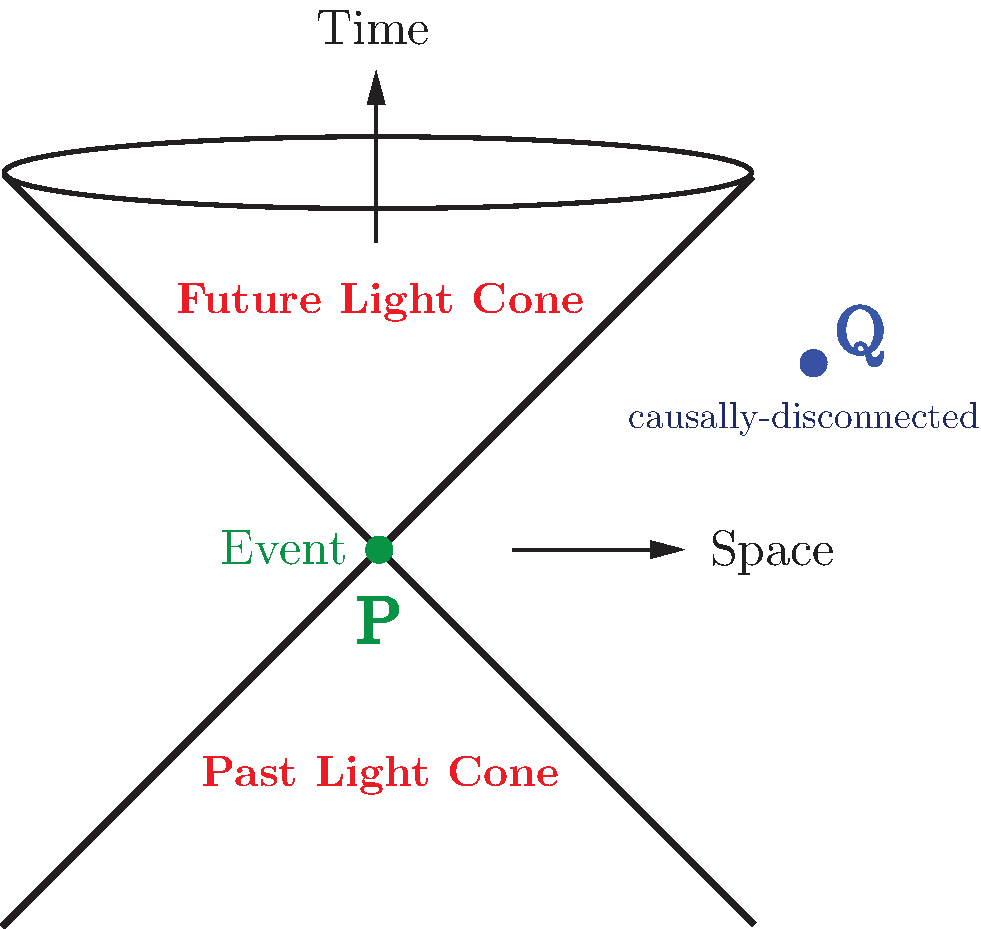
\includegraphics[width=.4\textwidth]{./lightcone}
        \caption{光円錐と因果律．光子は，{\it ヌル測地線}と呼ばれる，固有時間がゼロの世界線$\d s^2 =0$に沿って進む．
質量を持つ粒子は，{\it 時間的測地線}と呼ばれる，実数の固有時間を持つ世界線$\d s^2 > 0$に沿って進む．因果的につながっていない時空の領域は，{\it 空間的}な間隔$\d s^2 < 0$で隔てられる．時空のある点（あるいは{\it 事象}）を通るすべてのヌル測地線の集合を，{\it 光円錐}という．すべてのヌル測地線と時間的測地線からなる光円錐の内部が，その事象と因果的に関係する時空の領域を定める．}
    \label{fig:lightcone}
\end{figure}





%\vskip 6pt
%\noindent
\subsubsection*{粒子地平線}

初期時刻$t_{\rm i}$から，その後のある時刻$t$までの間に光が伝播できる最大の共動距離は，
\beq
\chi_p(\tau) = \tau - \tau_{\rm i} = \int_{t_{\rm i}}^t \frac{\d t}{a(t)}\, .
\eeq
である．これを（共動）粒子地平線と呼ぶ．初期時刻$t_{\rm i}$はしばしば，初期特異点$a(t_{\rm i} \equiv 0) \equiv 0$で定義される「宇宙の始まり」$t_{\rm i} \equiv 0$に取る．\footnote{$t_{\rm i} = 0$が$\tau_{\rm i} = 0$にも対応するかどうかは，スケール因子$a(t)$の進化に依存する．例えば，インフレーションでは$t_{\rm i}=0$は$\tau_{\rm i}=0$には{\it ならない}．}
粒子地平線の物理的な大きさは
\beq
d_p(t) = a(t) \chi_p\, .
\eeq
である．粒子地平線は，宇宙の因果構造の理解に決定的に重要であり，インフレーションの議論の基礎となる．
後に見るように，通常のビッグバン模型は過去の有限の時刻に「始まり」，過去のどの時点でも粒子地平線は有限であった．そのため，時空の領域同士が因果的に接触できた距離には限りがあった．
この特徴が「ビッグバンの謎」の核心にある．

%\vskip 6pt
%\newpage
%\noindent
\subsubsection*{事象の地平線}

事象の地平線は，ある時刻$\tau$に送られた信号が，将来にわたって観測者に届くことのない点の集合を定める．
共動座標では，これらの点は次を満たす．
\beq
\chi \ >\  \chi_e = \int_\tau^{\tau_{\rm max}} \d \tau = \tau_{\rm max} - \tau\, ,
\eeq
ここで$\tau_{\rm max}$は「時間の最後の瞬間」を表す（これは無限でも有限でもよい）．
事象の地平線の物理的な大きさは次のとおりである．
\beq
d_e(t) = a(t) \chi_e\, .
\eeq

%\vskip 6pt
%\noindent
\subsubsection*{角径距離と光度距離}

共形時間（または共動距離）は，角径距離および光度距離と簡単な関係にある．これらはそれぞれ，CMB異方性と超新星の距離を論じる際に重要である．
ここではその詳細には立ち入らないが，標準的な教科書\cite{Dodelson, Mukhanov, WeinbergCosmology}に説明がある．



\subsectionlink{力学：アインシュタイン方程式}
\label{sec:EinsteinEqns}

FRW時空のスケール因子$a(t)$の進化によって特徴付けられる宇宙の力学は，アインシュタイン方程式によって決まる．
\beq
\label{equ:Einstein}
\fbox{$\displaystyle
G_{\mu \nu} =8\pi G\, T_{\mu \nu} $}\, .
\eeq
以下ではしばしば，$8\pi G \equiv 1$となる単位系を用いる．

\subsubsection*{アインシュタイン重力}

便宜のため，ここでアインシュタイン・テンソルの定義を確認しておく．
\beq
G_{\mu \nu} \equiv R_{\mu \nu} - \frac{1}{2} g_{\mu \nu} R\, ,
\eeq
ここに現れるリッチ・テンソル$R_{\mu \nu}$とリッチ・スカラー$R$は，
\beq
R_{\mu \nu} = \Gamma^\alpha_{\ \mu \nu, \alpha} - \Gamma^\alpha_{\mu \alpha, \nu} + \Gamma^\alpha_{\ \beta \alpha} \Gamma^\beta_{\mu \nu} - \Gamma^\alpha_{\beta \nu} \Gamma^\beta_{\mu \alpha}\, , \qquad  R \equiv g^{\mu \nu} R_{\mu \nu}\, ,
\eeq
であり，
\beq
\Gamma^\mu_{\ \alpha \beta} \equiv \frac{g^{\mu \nu}}{2} \left[ g_{\alpha \nu , \beta} + g_{\beta \nu , \alpha} - g_{\alpha \beta, \nu}\right]\, .
\eeq
である．コンマは偏微分を表す．例えば，$(\dots)_{,\mu} =\frac{\partial (\dots)}{\partial x^\mu}$である．本講義では，以下もこの記法を用いる．

\subsubsection*{エネルギー，運動量，および圧力}

宇宙のエネルギー運動量テンソル$T_{\mu \nu}$を定義するため，世界線が次の時間的な4元速度ベクトルに接する観測者の集合を導入する．
\beq
u^\mu \equiv \frac{d x^\mu}{d \tau}\, ,
\eeq
ここで$\tau$は観測者の固有時間であり，$g_{\mu \nu} u^\mu u^\nu = -1$を満たす．
$u_\mu$に直交する3次元空間切片の計量として，テンソル$\gamma_{\mu \nu} \equiv g_{\mu \nu} + u_\mu u_\nu$を定義する．$\gamma_{\mu \nu}$を用い，諸量を4元速度に直交する，観測者の瞬間的な静止空間へ射影する．
すると，一般の（非完全）流体のエネルギー運動量テンソルは，次のように書ける．
\beq
T_{\mu \nu} = \rho u_\mu u_\nu + p \gamma_{\mu \nu} + 2 q_{(\mu} u_{\nu)} + \Sigma_{\mu \nu}\, ,
\eeq
ここで，$\rho = T_{\mu \nu} u^\mu u^\nu$は物質のエネルギー密度，$p = \frac{1}{3} T_{\mu \nu} \gamma^{\mu \nu}$は等方的圧力，$q_\mu = - \gamma_\mu^{\ \alpha} T_{\alpha \beta} u^\beta$はエネルギー流束ベクトル，$\Sigma_{\mu \nu} = \gamma_{\langle \mu}^{\ \alpha} \gamma_{\nu \rangle}^{\ \beta} T_{\alpha \beta}$は対称かつトレースレスな異方的応力テンソルである．\footnote{ここでは，$t_{\langle \mu \nu \rangle} = \gamma_{(\mu}^{\ \alpha} \gamma_{\nu)}^{\ \beta} t_{\alpha \beta} - \frac{1}{3} \gamma^{\alpha \beta} t_{\alpha \beta} \gamma_{\mu \nu}$および$t_{(\mu \nu)} = \frac{1}{2}(t_{\mu \nu}+t_{\nu \mu})$という記法を用いる．}
完全流体の場合，$q_\mu = \Sigma_{\mu \nu} = 0$となる4元速度が一意に存在する．すなわち，完全流体のエネルギー運動量テンソルは
\beq
T^\mu_{\ \nu} = g^{\mu \alpha} T_{\alpha \nu} = (\rho + p) \, u^\mu u_\nu - p\, \delta^\mu_\nu \, ,
%= \left( \begin{array}{cccc} \rho & 0 & 0 & 0\\ 0 & - p&0 &0 \\ 0& 0&-p&0 \\ 0&0&0& - p \end{array} \right)\, ,
\eeq
である．ここで$\rho$と$p$は流体の静止系における固有エネルギー密度と圧力であり，$u^\mu$は流体の4元速度である．
%The 4-velocity satisfies $g_{\mu \nu} u^\mu u^\nu = -1$.
流体と共動する座標系では，$u^\mu = (1,0,0,0)$と選べる．すなわち，
\beq
\label{equ:pf}
T^\mu_{\ \nu} = \left( \begin{array}{cccc} \rho & 0 & 0 & 0\\ 0 & - p&0 &0 \\ 0& 0&-p&0 \\ 0&0&0& - p \end{array} \right)\, .
\eeq
このときアインシュタイン方程式は，2本の結合した非線形常微分方程式の形になる．これらを{\it フリードマン方程式}とも呼ぶ（{\bf 問題~\ref{pro:Friedmann}}参照）．
\beq
\label{equ:Fried}
\fbox{$\displaystyle
H^2 \equiv \left(\frac{\dot a}{a}\right)^2 =  \frac{1}{3} \rho - \frac{k}{a^2}  $}\, ,
\eeq
および
\beq
\label{equ:Ray}
\fbox{$\displaystyle
\dot H + H^2 = \frac{\ddot a}{a} =  - \frac{1}{6} (\rho + 3 p) $}\, ,
\eeq
%Here we defined the Hubble parameter $H \equiv \partial_t \ln a$ as a measure of the expansion rate of the universe.
ここで，上付きのドットは物理的時間$t$に関する微分を表す．
通常の物質（すなわち強いエネルギー条件$\rho + 3 p \ge 0$を満たす物質）で満たされた膨張宇宙（すなわち$\dot a > 0$）では，式~(\ref{equ:Ray})が$\ddot a < 0$を意味することに注意しよう．これは，有限の過去に特異点$a(t\equiv 0)=0$が存在することを示す．もちろん，この結論は，一般相対性理論とフリードマン方程式が任意に高いエネルギーまで適用でき，高エネルギーで特異な形態の物質が重要にならないという仮定に依存する．
むしろ特異点は，一般相対性理論の破綻を示していると考える方が自然である．

式~(\ref{equ:Fried})と式~(\ref{equ:Ray})を組み合わせると，連続の式を得る．
\beq
\fbox{$\displaystyle
\frac{d \rho}{dt} +  3 H (\rho + p) = 0 $}\, .
\eeq
これは，次のようにも書ける．
\beq
\label{equ:conXXX}
\frac{d \ln \rho}{d \ln a} = - 3(1+w)\, ,
\eeq
ただし，状態方程式パラメータを
\beq
w \equiv \frac{p}{\rho}\, .
\eeq
と定義した．式~(\ref{equ:conXXX})を積分すると，
\beq
\rho \propto a^{-3(1+w)}\, .
\eeq
となる．これをフリードマン方程式(\ref{equ:Fried})と合わせると，スケール因子の時間発展が得られる．
\beq
a(t) \propto \left\{ \begin{array}{lc} t^{2/3(1+w)}\quad & \ w \ne -1\, , \\
e^{Ht}\quad & \ w = -1\, ,
\end{array} \right.
\eeq
すなわち，非相対論的物質（$w=0$），放射または相対論的物質（$w=\frac{1}{3}$），宇宙定数（$w=-1$）がそれぞれ支配する平坦な（$k=0$）宇宙のスケール因子は，順に$a(t)\propto t^{2/3}$，$a(t)\propto t^{1/2}$，$a(t)\propto \exp(Ht)$となる．

\begin{table}[h!]
\caption{放射，物質，または宇宙定数が支配する平坦な宇宙のFRW解．}
\label{tab:solutions}
\begin{center}
\vspace{-0.7cm}
\begin{tabular}{| l |  c | c | c | c | c|}
\hline
 & $w$ & $\rho(a) $ & $a(t)$ & $a(\tau)$ & $\tau_{\rm i}$ \\
\hline
\hline
物質優勢（MD） & 0 & $a^{-3}$ & $t^{2/3}$ & $\tau^2$ & 0\\
放射優勢（RD） & $\frac{1}{3}$ & $a^{-4}$ & $t^{1/2}$ & $\tau$ &0  \\
$\Lambda$ & $-1$ & $a^0$ & $e^{Ht}$ & $- \tau^{-1}$ & $- \infty$ \\
\hline
\end{tabular}
\end{center}
\end{table}

複数の種類の成分（バリオン，光子，ニュートリノ，ダークマター，ダークエネルギーなど）がエネルギー密度と圧力に有意に寄与する場合，$\rho$と$p$はすべての成分の和を表す．
\beq
\rho \equiv \sum_{i} \rho_{i}\, , \qquad p \equiv \sum_{i} p_{i}\, .
\eeq
各成分「${i}$」について，そのエネルギー密度の，{\it 臨界エネルギー密度}$\rho_{\rm crit} \equiv 3 H_0^2$に対する{\it 現在}の比を
\beq
\Omega_{i} \equiv {\rho_0^{i} \over \rho_{\rm crit}}\, ,
\eeq
と定義し，対応する状態方程式を
\beq
w_{i} \equiv {p_{i} \over \rho_{i}}\, .
\eeq
とする．ここで，また以下でも，添字「0」はある量を現在時刻$t_0$で評価することを表す．
スケール因子を$a_0  = a(t_0) \equiv 1$となるように規格化する．
これにより，フリードマン方程式(\ref{equ:Fried})は次のように書ける．
\beq
\label{equ:FriedX}
\left({H\over H_0}\right)^2=\sum_i\Omega_{i}
a^{-3(1+w_{i})}+\Omega_k
a^{-2},
\eeq
ここで$\Omega_k \equiv -k/a_0^2H_0^2$が曲率をパラメータ化する．
式~(\ref{equ:FriedX})を現在で評価すると，次の整合性関係を得る．
\beq
\sum_i \Omega_{i}+\Omega_k=1\, .
\eeq
第2フリードマン方程式(\ref{equ:Ray})を$t=t_0$で評価すると，
\beq
{1 \over a_0 H_0^2} {d^2 a_0 \over d t^2}=-{1\over 2}\sum_i \Omega_{i}(1+3 w_{i}).
\eeq
となる．これが，現在の加速膨張の条件を定める．



\subsectionlink{コンコーダンス模型}

 \begin{figure}[h!]
    \centering
        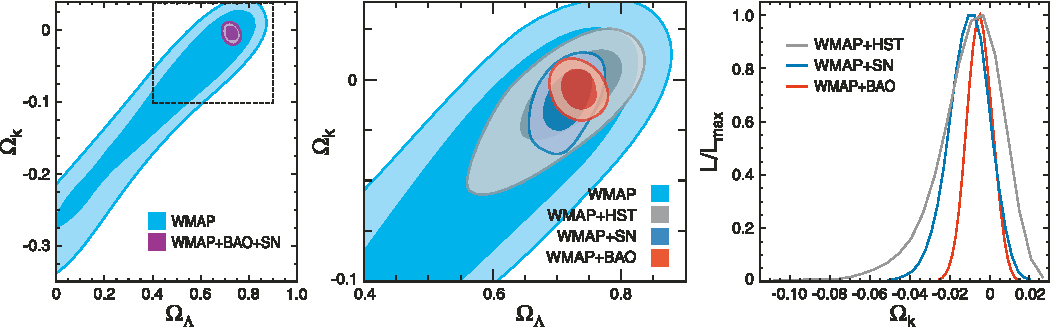
\includegraphics[width=.9\textwidth]{./KomatsuFlat}
        \caption{CMBとLSSの観測を組み合わせると，宇宙の空間的な幾何は平坦であることが示される\cite{WMAP5}．平坦性の証拠は，CMB観測だけからは得られないことに注意しよう．}
    \label{fig:flat}
\end{figure}

宇宙マイクロ波背景放射と大規模構造の観測から，宇宙は平坦であることが分かる（図~\ref{fig:flat}参照）．
\beq
\Omega_k \sim 0\, ,
\eeq
また，その構成は原子（またはバリオン「$b$」）が4\%，（冷たい）ダークマター（「$dm$」）が23\%，ダークエネルギー（$\Lambda$）が73\%である（図~\ref{fig:concord}参照）．
 \beq
 \Omega_b = 0.04\, , \ \ \Omega_{dm} = 0.23\, , \ \  \Omega_{\Lambda} = 0.72\, ,
 \eeq
ここで$w_\Lambda \approx -1$である（図~\ref{fig:concord2}参照）．
% \vspace{-1cm}
\begin{figure}[h!]
    \centering
        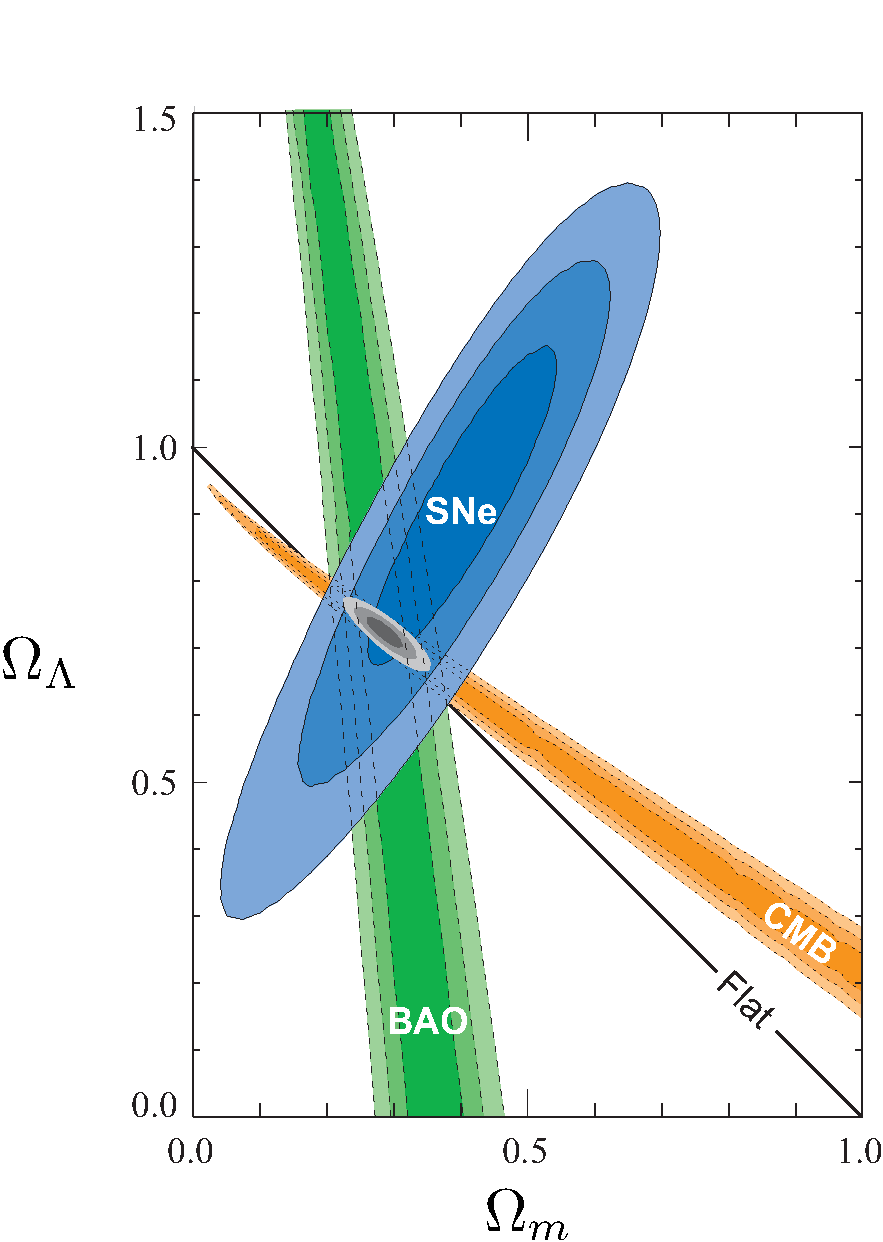
\includegraphics[width=.4\textwidth]{./DEkosowski}
        \caption{ダークエネルギーの証拠．宇宙マイクロ波背景放射（CMB），超新星（SNe），およびバリオン音響振動（BAO）の観測を組み合わせたものを示す\cite{unionsn}．}
    \label{fig:concord}
\end{figure}
 
 \begin{figure}[h!]
    \centering
        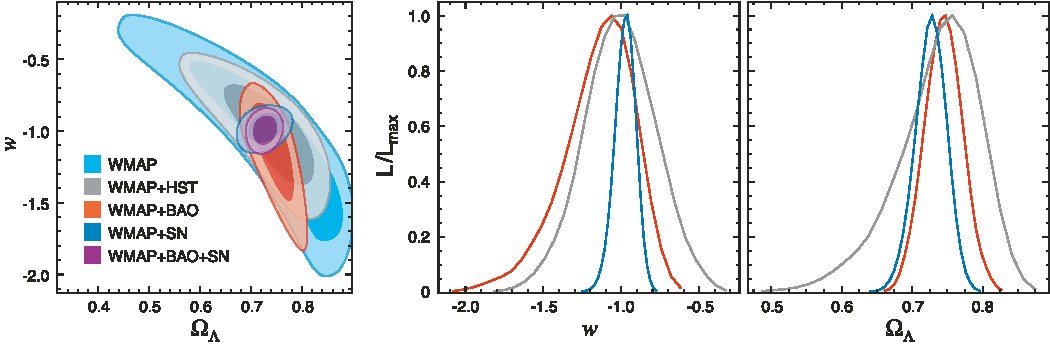
\includegraphics[width=.9\textwidth]{./KomatsuDE}
        \caption{ダークエネルギーの性質は宇宙定数に近く，$w_\Lambda \approx -1$である\cite{WMAP5}．}
    \label{fig:concord2}
\end{figure}

さらに宇宙には，断熱的でスケール不変，かつガウス的な密度揺らぎの微小なさざ波が存在することも分かっている．
%What is the physical origin of these primordial perturbations to the homogeneous universe?
本連続講義の大部分では，インフレーション中の量子揺らぎが，観測される宇宙論的摂動をどのように説明できるかを述べる．






%more than one component


%It useful to define the critical density of a flat ($k=0$) universe, $\rho_{\rm crit} = 3 H^2$.

%Define $\Omega$
\newpage
\sectionlink{ビッグバンの謎}


初期条件が物理理論の一部をなすのか，それとも別に考えるべきなのかは，いくらか哲学的な問いである．
物理学の目的は，一組の初期条件が与えられたとき，系のその後の進化を予言することにある．例えば，物体の初期位置と初期速度を定めれば，ニュートンの重力法則はその軌道を予言する．
したがって，宇宙論が宇宙の初期条件を予言すべきか，あるいは単に説明すべきかすら，決して明らかではない．
一方で，極めて特殊で微調整された初期条件からしか，私たちが見ているような宇宙が生まれず，観測される宇宙が「起こりそうもない偶然」であるとしたら，それは非常に残念なことである．

本節では，通常のビッグバン理論が，宇宙を現在の状態へ進化させるために，まさにそのような微調整された初期条件を必要とすることを説明する．
インフレーションの主要な成果の一つは，宇宙の初期条件を説明することである．
インフレーションを通じて，私たちにとって身近で大切な宇宙は，一般的な初期条件から成長した．

\subsectionlink{宇宙のコーシー問題}

宇宙の初期条件を指定するために，一定時刻の空間切片$\Sigma$を考える（ここでは，$\Sigma$の選び方のゲージ依存性は気にしない）．
3次元超曲面$\Sigma$上で，すべての物質粒子の位置と速度を定義する．
次に重力と流体力学の法則を用いて，系を時間の進む向きに発展させる．


\begin{itemize}
\item 初期の一様性

物質の空間分布を，座標${\bf x}$の関数としての密度と圧力，すなわち$\rho({\bf x})$と$p({\bf x})$で記述する．
前節では宇宙の一様性と等方性を仮定した．なぜこれはよい仮定なのだろうか．%This is particularly surprising given that i
非一様性は重力的に不安定であり，したがって時間とともに成長する．宇宙マイクロ波背景放射の観測は，過去（最終散乱時）の非一様性が，現在よりはるかに小さかったことを示している．したがって，さらに早い時刻には，これらの非一様性はもっと小さかったと予想される．
初期宇宙の滑らかさを，どう説明すればよいだろうか．

これは特に驚くべきことである．というのも，\S\ref{sec:horizon}で示すように，通常のビッグバン描像では，初期宇宙（例えば最終散乱時のCMB）は，因果的につながっていない多数の空間領域からなっていたからである．ビッグバン理論には，これらの因果的に隔てられた領域が，なぜこれほど似た物理的状況を示すのかを説明する力学的理由がない．
このため一様性の問題は，しばしば{\it 地平線問題}と呼ばれる．

\item 初期速度

宇宙のコーシー問題を完全に指定するには，初期密度分布に加えて，空間の各点における流体の速度が必要である．
後に見るように，宇宙が後期にも一様なままであることを保証するには，初期の流体速度が極めて精密な値を取らなければならない．
初期速度がわずかに小さすぎるだけで，宇宙は1秒もたたないうちに再崩壊する．
わずかに大きすぎるだけで，宇宙は急速に膨張しすぎ，たちまちほぼ空になってしまう．
この初期速度の微調整は，地平線問題と組み合わせて考えると，さらに際立つ．因果的に隔てられた空間領域にわたって，流体速度を微調整しなければならないのである．

ポテンシャルエネルギーと運動エネルギーの差が，空間領域の局所的な曲率を定めるため（{\bf 演習~\ref{ex:flatness}}参照），この初期速度の微調整は，しばしば{\it 平坦性問題}と呼ばれる．

\end{itemize}

\subsectionlink{地平線問題}
\label{sec:horizon}

前節では，{\it 共動（粒子）地平線}$\tau$を，因果的地平線，すなわち時刻$0$から時刻$t$までに光線が進める最大距離として定義した．
\beq
\fbox{$\displaystyle
\tau \equiv \int_0^t \frac{\d t'}{a(t')} = \int_0^a \frac{\d a}{Ha^2} = \int_0^a \d \ln a \left(\frac{1}{aH}\right)$}\, .
\eeq
ここでは共動地平線を，インフレーションで決定的な役割を果たす{\it 共動ハッブル半径}$(aH)^{-1}$の積分として表した．

状態方程式$w$を持つ流体が支配する宇宙では，次が成り立つ．
\beq
(aH)^{-1} = H_0^{-1} a^{\frac{1}{2}(1+3w)}\, .
\eeq 
指数が組合せ$(1+3w)$に依存することに注意しよう．
したがって，その定性的な振る舞いは，$(1+ 3 w)$が正か負かによって変わる．
%The comoving Hubble radius 
%I will show in a moment that the {\it comoving Hubble radius}, $(aH)^{-1}$, characterizes
%the fraction of comoving space in causal contact.
通常のビッグバン膨張（$w \gtrsim 0$）では，$(a H)^{-1}$は単調に{\it 増大}し，共動地平線$\tau$，すなわち{\it 因果的に接触している宇宙の割合は時間とともに増える}．
\beq
\tau \propto a^{\frac{1}{2}(1+ 3 w)}\, .
\eeq
ここでも，定性的な振る舞いは$(1+3w)$が正か負かによって変わる．
特に，放射優勢（RD）および物質優勢（MD）の宇宙について，次を得る．
\beq
\tau = \int_0^a \frac{\d a}{Ha^2} \propto
\left\{ 
\begin{array}{ll}
a \quad \quad \,\rm{RD}\\
a^{1/2} \quad \rm{MD}
\end{array} \right.  \, . 
\eeq
これは，共動地平線が時間とともに単調に増大することを意味する．したがって，現在地平線へ入ってくる共動スケールは，CMB脱結合時には地平線のはるか外にあったことになる．\footnote{揺らぎの共動波長は時間に依存しないのに対し，共動ハッブル半径は時間に依存することを思い出そう．}
%Why is the CMB uniform on large scales (of order the present horizon)?
ところがCMBがほぼ一様であることは，最終散乱の時点において，{\it 先験的には}因果的に独立しているはずの多くの領域を含むスケールにわたって，宇宙が極めて一様だったことを示している．
これはどうして可能なのだろうか．

%To be more specific,
%consider radial null geodesics in a flat FRW spacetime
%\beq
%\d s^2 = \d t^2 - a(t)^2 \d r^2 \equiv 0 \quad \quad \Rightarrow \quad \quad \d r = \pm \frac{\d t}{a(t)} \equiv \d \tau\, .
%\eeq
%We define the
%{\it comoving horizon}, $\tau$, as the causal horizon or the maximum distance a light ray can travel between time $0$ and time $t$
%\beq
%\fbox{$\displaystyle
%\tau \equiv \int_0^t \frac{\d t'}{a(t')} = \int_0^a \frac{\d a}{Ha^2} = \int_0^a \d[\ln a] \left(\frac{1}{aH}\right)$}\, .
%\eeq
%During the standard cosmological expansion the increasing comoving Hubble radius, $\frac{1}{aH}$, is therefore associated with an increasing comoving horizon\footnote{This justifies the common practice of often using the terms 'comoving Hubble radius' and 'comoving horizon' interchangeably. Although these terms should conceptually be clearly distinguished, this inaccurate use of language has become standard.}, $\tau$. In particular for radiation dominated (RD) and matter dominated (MD) universes we find
%\begin{eqnarray}
%\tau &=& \int_0^a \frac{\d a}{Ha^2} \nonumber\\
%&=& \frac{1}{H_0} \int_0^a \frac{\d a}{\Omega^{1/2}(a) a^2} \nonumber\\
%&\propto& 
%\left\{ 
%\begin{array}{ll}
%a \quad \quad \,\rm{RD}\\
%a^{1/2} \quad \rm{MD}
%\end{array} \right.  \, . 
%\end{eqnarray}
%This means that the comoving horizon grows monotonically with time (at least in an expanding universe) which implies that comoving scales entering the horizon today have been far outside the horizon at CMB decoupling.
%Why is the CMB uniform on large scales (of order the present horizon)?


\subsectionlink{平坦性問題}
\label{sec:flatness}

\begin{thm}[平坦性と運動エネルギー]
曲率パラメータ$$\Omega_k \equiv \Omega - 1= \frac{\rho-\rho_{\rm crit}}{\rho_{\rm crit}}\, , \qquad \text{ただし} \quad \rho_{\rm crit} \equiv 3 H^2\, ,$$が，空間のある領域の平均ポテンシャルエネルギーと平均運動エネルギーの差として解釈できることを示せ．
\label{ex:flatness}
\end{thm}

%{\tt Fix}

一般相対性理論の時空は力学的なものであり，宇宙の物質に応答して曲がる．それなら，なぜ宇宙は平坦なユークリッド空間でこれほどよく近似されるのだろうか．
この問題を定量化するため，フリードマン方程式を考える．
\begin{equation}
H^2 = \frac{1}{3} \rho(a) - \frac{k}{a^2}\, ,
\end{equation}
これを次のように書く．
\begin{equation}
\label{equ:omega}
\fbox{$\displaystyle
1-\Omega(a) = \frac{-k}{(aH)^2}$}\, ,
\end{equation}
ここで，
\begin{equation}
\Omega(a) \equiv \frac{\rho(a)}{\rho_{\rm crit}(a)}\, , \qquad \rho_{\rm crit}(a) \equiv 3 H(a)^2\, .
\end{equation}
である．ここでは$\Omega(a)$を時間依存する量として定義しているのに対し，前節までの$\Omega$は定数$\Omega(a_0)$であったことに注意しよう．
標準宇宙論では，共動ハッブル半径$(aH)^{-1}$は時間とともに増大するので，式~(\ref{equ:omega})から，$|\Omega-1|$も時間とともに発散しなければならない．臨界値$\Omega=1$は{\it 不安定な固定点}である．したがって，インフレーションを含まない標準ビッグバン宇宙論では，現在観測されるほぼ平坦な状態$\Omega(a_0) \sim 1$を実現するには，初期宇宙の$\Omega$を$1$の極めて近くに微調整する必要がある．
より具体的には，ビッグバン元素合成（BBN）の時期，大統一（GUT）期，およびプランク・スケールにおける平坦性からのずれは，それぞれ次の条件を満たさなければならない．
\begin{eqnarray}
|\Omega(a_{\rm BBN})-1| &\le& {\cal O}(10^{-16})\, ,\\
|\Omega(a_{\rm GUT})-1| &\le& {\cal O}(10^{-55})\, ,\\
|\Omega(a_{\rm pl})-1| &\le& {\cal O}(10^{-61})\, .
\end{eqnarray}

平坦性問題は，次の微分方程式から理解することもできる．
\begin{equation}
\label{equ:omega2}
\frac{d \Omega}{d \ln a} = (1+3w) \Omega (\Omega-1)\, .
\end{equation}
式~(\ref{equ:omega2})は，式~(\ref{equ:omega})を微分し，連続の式(\ref{equ:conXXX})を使って導かれる．これにより，強いエネルギー条件が満たされる場合には，$\Omega=1$が不安定な固定点であることが明らかになる．
\begin{equation}
\frac{d |\Omega-1|}{d \ln a} > 0 \quad \Leftrightarrow \quad 1+3w > 0\, .
\end{equation}
改めて問おう．なぜ$\Omega(a_0) \sim {\cal O}(1)$なのであって，それよりはるかに小さくも，大きくもないのだろうか．


\subsectionlink{初期条件問題について}

平坦性問題と地平線問題は，標準宇宙模型の厳密な不整合では{\it ない}ことを強調しておこう．$\Omega$の初期値が極めて1に近く，宇宙が地平線を超える距離にわたって一様に始まったと仮定すれば（ただし，構造形成を説明するのにちょうど適切な程度の非一様性を伴っていれば），宇宙は観測と一致するように，一様なまま進化し続ける．したがって，平坦性問題と地平線問題は，実際にはビッグバン模型の予言能力における深刻な欠点である．初期宇宙の驚くほどの平坦性は，標準模型から予言することができず，初期条件として仮定しなければならない．同様に，宇宙の大きなスケールでの著しい一様性も，模型によって説明も予言もされず，単に仮定しなければならない．
これらの初期条件を力学的に説明する理論は，非常に魅力的に思われる．


\sectionlink{インフレーションへの第一歩}

%\subsectionlink{Solution of the Big Bang Puzzles}

\subsectionlink{縮むハッブル球}

\S\ref{sec:horizon}と\S\ref{sec:flatness}では，標準ビッグバン宇宙論の地平線問題と平坦性問題において，共動ハッブル半径$(a H)^{-1}$が果たす根本的な役割を強調した．
どちらの問題も，通常の宇宙論では共動ハッブル半径が厳密に増大することから生じる．これは，美しいほど単純な発想によって，ビッグバンの謎をすべて解けることを示唆する．
すなわち，{\it 共動ハッブル半径の振る舞いを反転させる}，つまり{\it 極初期宇宙で共動ハッブル半径を十分に減少させる}のである．

\subsubsection{インフレーション中の共動地平線}

共動地平線の進化は，インフレーションの考え方全体にとって極めて重要なので，いくつかの重要な点を明確に述べておく価値がある．

共動地平線（＝共形時間）の定義が，共動ハッブル半径の対数積分であることを思い出そう．
\beq
\label{equ:tau}
\fbox{$\displaystyle
\tau = \int_0^a \d \ln a' \ \frac{1}{a' H(a')} $}\, .
\eeq

共動地平線$\tau$と共動ハッブル半径$(aH)^{-1}$の微妙な違いを強調しておこう\cite{Dodelson}．
\begin{quote}
粒子が$\tau$より大きな距離で隔てられていれば，それらは{\it 一度も}互いに情報をやり取りできなかった．粒子が$(aH)^{-1}$より大きな距離で隔てられていれば，それらは{\it 今}は情報をやり取りできない！ この違いは，地平線問題の解決に決定的であり，その解決は次の点に依拠する．現在の$\tau$が$(aH)^{-1}$よりはるかに大きければ，粒子は今日情報をやり取りできなくても，初期には因果的に接触していたことがありうる．式~(\ref{equ:tau})から，初期宇宙の共動ハッブル半径が現在よりもはるかに大きく，$\tau$への寄与の大部分が初期から来る場合には，これが起こりうると分かる．したがって，ハッブル半径が減少する時期が必要である．
インフレーション中は$H$がほぼ一定のまま$a$が指数関数的に増大するため，共動ハッブル半径は，まさに述べたとおり減少する．
\end{quote}

インフレーション中に共動地平線が減少することは，ビッグバンの謎を解くだけでなく，第2講で述べる宇宙論的摂動の量子的生成に必要な，鍵となる特徴でもある．量子揺らぎは地平線より小さなスケールで生成されるが，ハッブル半径がその共動波長より小さくなると，地平線の外へ出ることを説明する．物理座標では，これは超光速の膨張が摂動を因果的につながらない距離まで引き伸ばすことに対応する．それらは地平線を超える古典的な密度摂動となり，その後のビッグバンの進化で地平線へ再突入してから，重力崩壊して宇宙の大規模構造を形成する．

インフレーション中に共動地平線と共動ハッブル半径がどのように進化するかを理解したので，インフレーションがビッグバンの謎を解く仕組みの説明は，もはやほとんど自明である．

\subsubsection{平坦性問題を再考する}

平坦でない宇宙に対するフリードマン方程式(\ref{equ:omega})を思い出そう．
\begin{equation}
|1-\Omega(a)| = \frac{1}{(aH)^2}\, .
\end{equation}
共動ハッブル半径が減少すると，宇宙は平坦性から遠ざかるのでなく，{\it 平坦性へと近づいていく}．
これで平坦性問題が解決する！ インフレーション中，解$\Omega=1$はアトラクターである．

\subsubsection{地平線問題を再考する}

共動地平線が減少するということは，現在の宇宙に入ってくる大きなスケールが，インフレーション以前には地平線の内側にあったことを意味する（図2参照）．したがって，インフレーション以前の因果的な物理過程が，空間的一様性を確立した．
インフレーション期があれば，CMBの一様性は謎ではない．

%explain 60 $e$-folds from fig 2.

\begin{figure}[h]
	\centering
		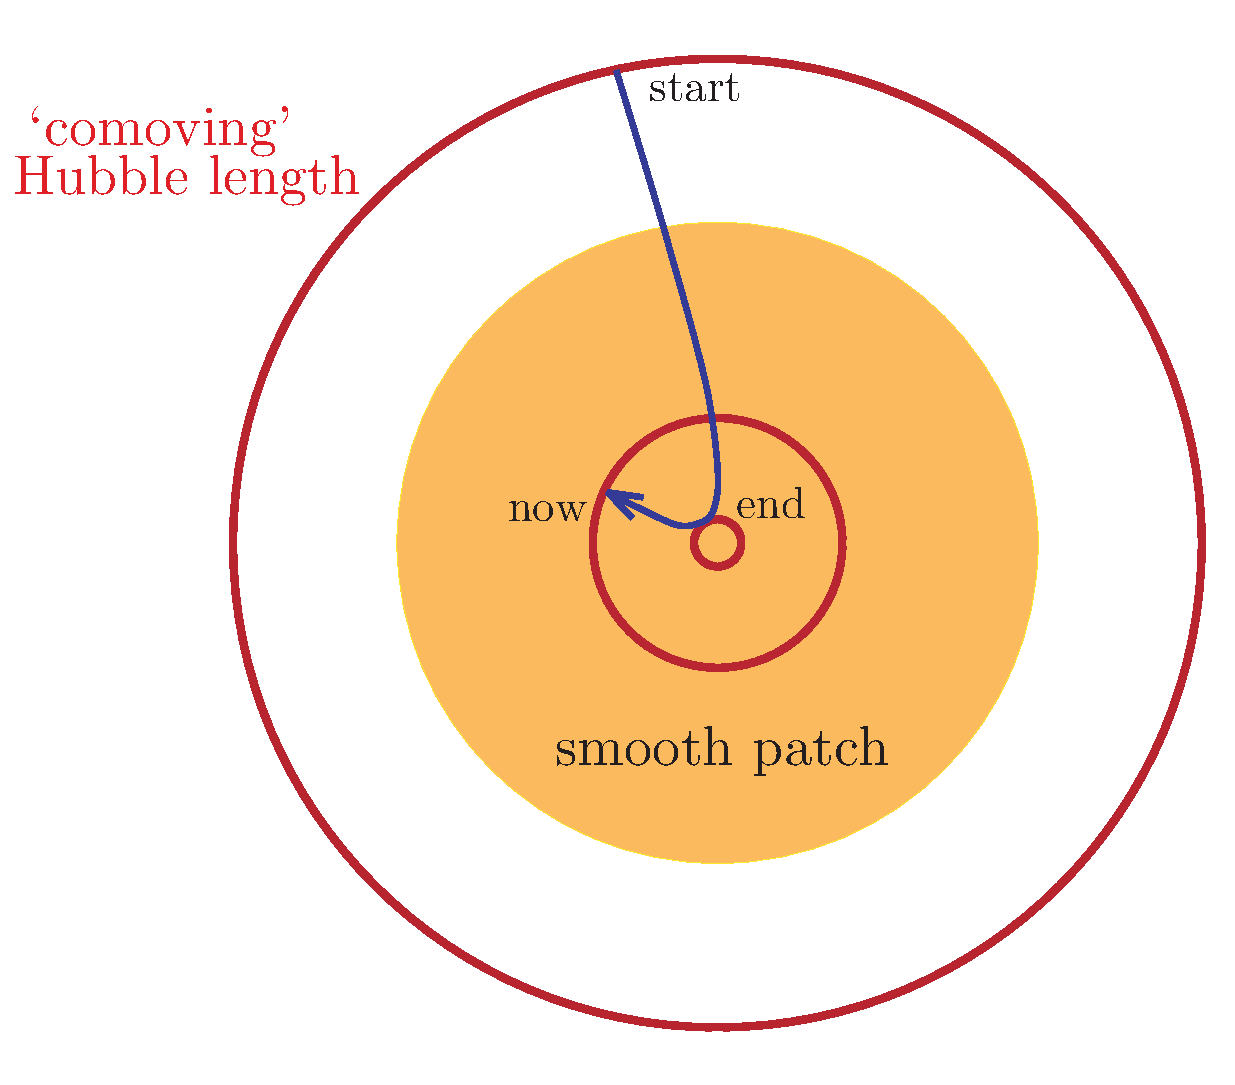
\includegraphics[width=6cm]{horizon}
		\hspace{0.5cm} 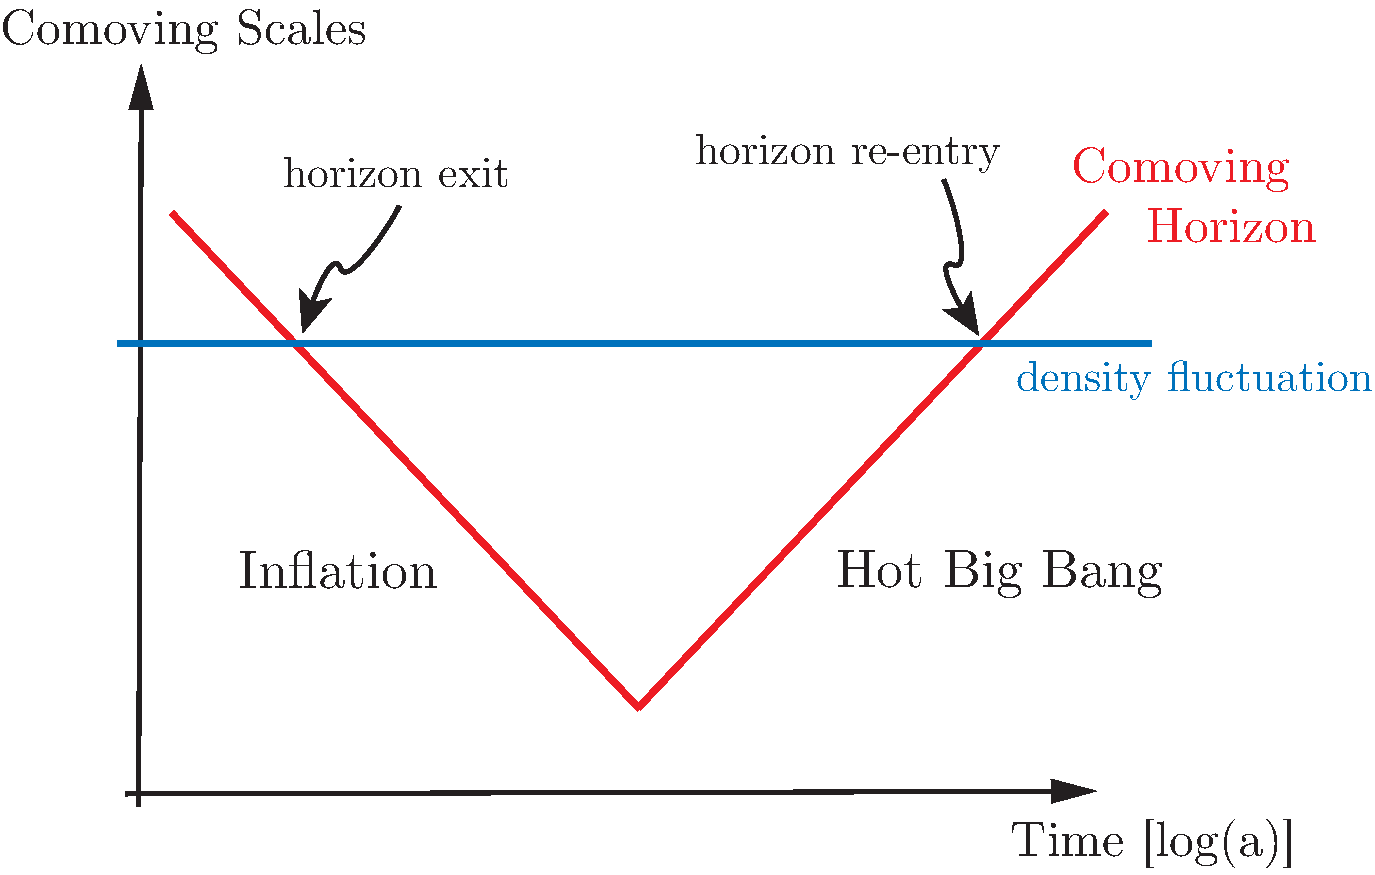
\includegraphics[width=8cm]{Scales}
	\label{fig:horizon}
\caption{{\it 左：}インフレーション宇宙における共動ハッブル半径$(aH)^{-1}$の進化．
	%[Figure adapted from Liddle and Lyth \cite{LiddleLyth}.] 
共動ハッブル球はインフレーション中に縮み，インフレーション後に膨張する．
したがってインフレーションは，地平線より小さな滑らかな領域を「拡大して見る」機構である．
{\it 右：}地平線問題の解決．今日の宇宙論的観測に関係するすべてのスケールは，$a\sim 10^{-5}$まではハッブル半径より大きかった．しかし，十分に早い時刻には，これらのスケールはハッブル半径より小さく，したがって因果的につながっていた．同様に，宇宙論的に関心のあるスケールは，比較的最近になってハッブル半径の内側に再び入ってきた．}
\end{figure}


\subsectionlink{インフレーションの条件}

フリードマン方程式を通じて，共動ハッブル半径の縮小は，宇宙の加速および圧力に関係付けられる．
\beq
\fbox{$\displaystyle
\frac{d}{d t} \left(\frac{H^{-1}}{a}\right) < 0 \quad \Rightarrow \quad {d^2 a \over d t^2} >0 \quad \Rightarrow \quad \rho+3p <0 $}\, .
\eeq
したがって，インフレーションの三つの同値な条件は次のとおりである．
\begin{itemize}
\item {\bf 共動地平線の減少}

縮小するハッブル球は，次の条件で定義される．
\beq
\frac{d}{d t} \left(\frac{1}{aH}\right) < 0\, .
\eeq
これをインフレーションの基本的な定義として用いたのは，平坦性問題と地平線問題に最も直接に関係し，揺らぎを生成する機構の鍵となるからである．

\item {\bf 加速膨張}

関係式
\beq
\frac{d}{d t} (a H)^{-1} = \frac{- \ddot a}{(a H)^2}\, ,
\eeq
から，共動ハッブル半径の縮小が加速膨張を意味することが直ちに分かる．
\beq
{d^2 a \over d t^2 } >0\, . 
\eeq
これが，インフレーションがしばしば加速膨張期と定義される理由である．
もちろんスケール因子の時間に関する2階微分は，ハッブル・パラメータ$H$の時間に関する1階微分に関係付けられる．
\beq
\frac{\ddot a}{a} = H^2 (1-\varepsilon)\, , \qquad \text{ただし} \quad \varepsilon \equiv  - \frac{\dot H}{H^2}\, .
\eeq
したがって加速は，次の条件に対応する．
\beq
\label{equ:eps}
\fbox{$\displaystyle
\varepsilon = - \frac{\dot H}{H^2} = - \frac{d \ln H}{d N}< 1 $}
\eeq
ここでは$\d N = H \d t = \d \ln a$と定義した．これは，インフレーションによる膨張の$e$-fold数$N$を測る．
したがって式~(\ref{equ:eps})は，1 $e$-fold当たりのハッブル・パラメータの相対変化が小さいことを意味する．

 
\item {\bf 負の圧力}

どのようなエネルギー運動量が，加速を引き起こせるだろうか．
式~(\ref{equ:Ray})を参照すると，$\ddot a > 0$には次が必要であると分かる．
\beq
p < - \frac{1}{3} \rho\, ,
\eeq
すなわち，負の圧力，あるいは強いエネルギー条件（SEC）の破れが必要である．
これが物理理論でどのように実現されるかは，\S\ref{sec:SR}で説明する．
SECは決して絶対的なものではなく，容易に破られうることが分かるだろう．
\end{itemize}


\subsectionlink{インフレーションの共形図}

\begin{figure}
	\centering
		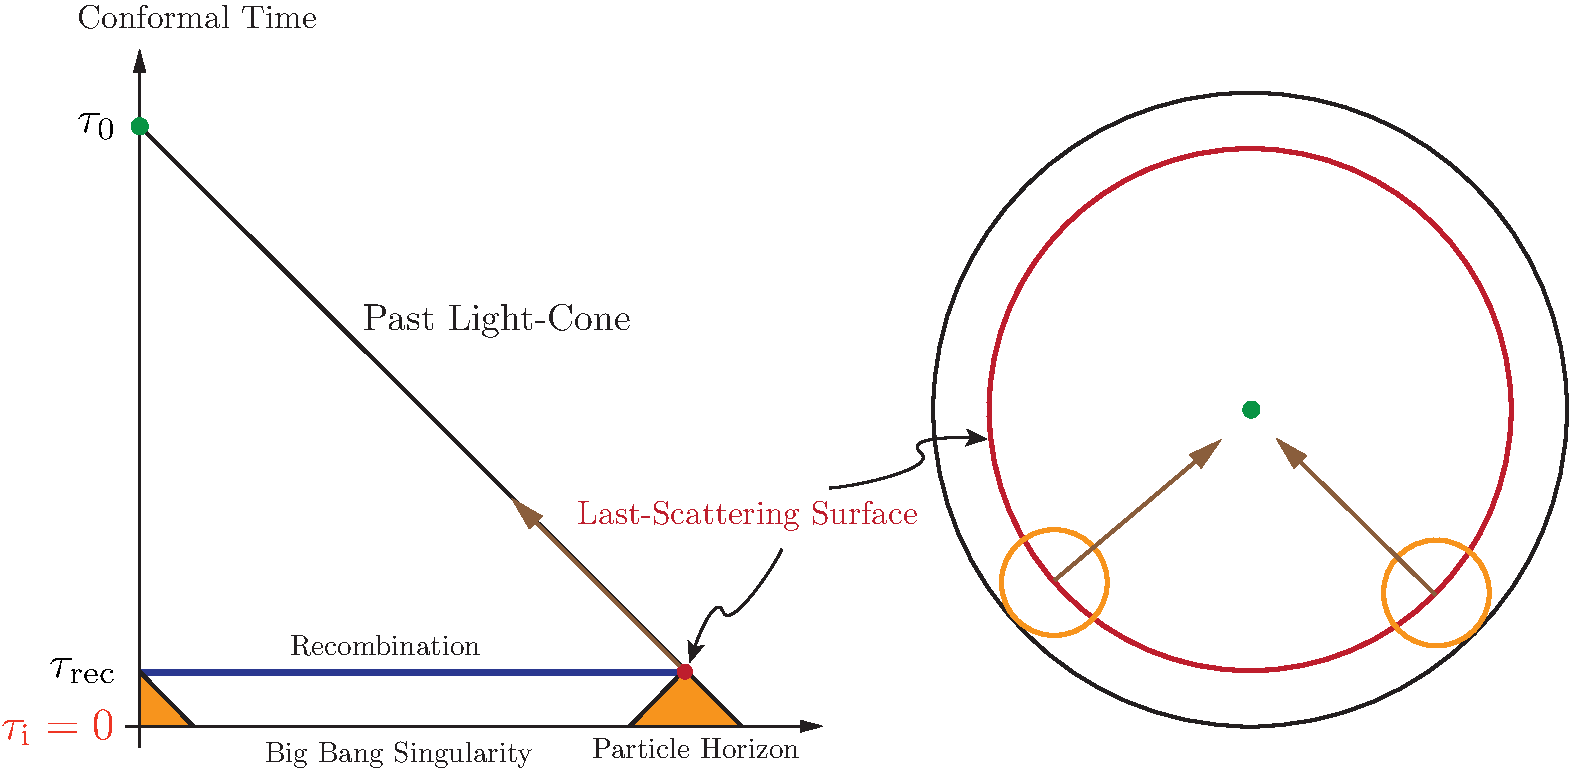
\includegraphics[width=0.98\textwidth]{FRWHorizon}
\caption{ビッグバン宇宙論の共形図．最終散乱（再結合）時のCMBは，因果的につながっていない$10^5$個の領域からなる！}
	\label{fig:Conformal1b}
\end{figure}
\begin{figure}
	\centering
		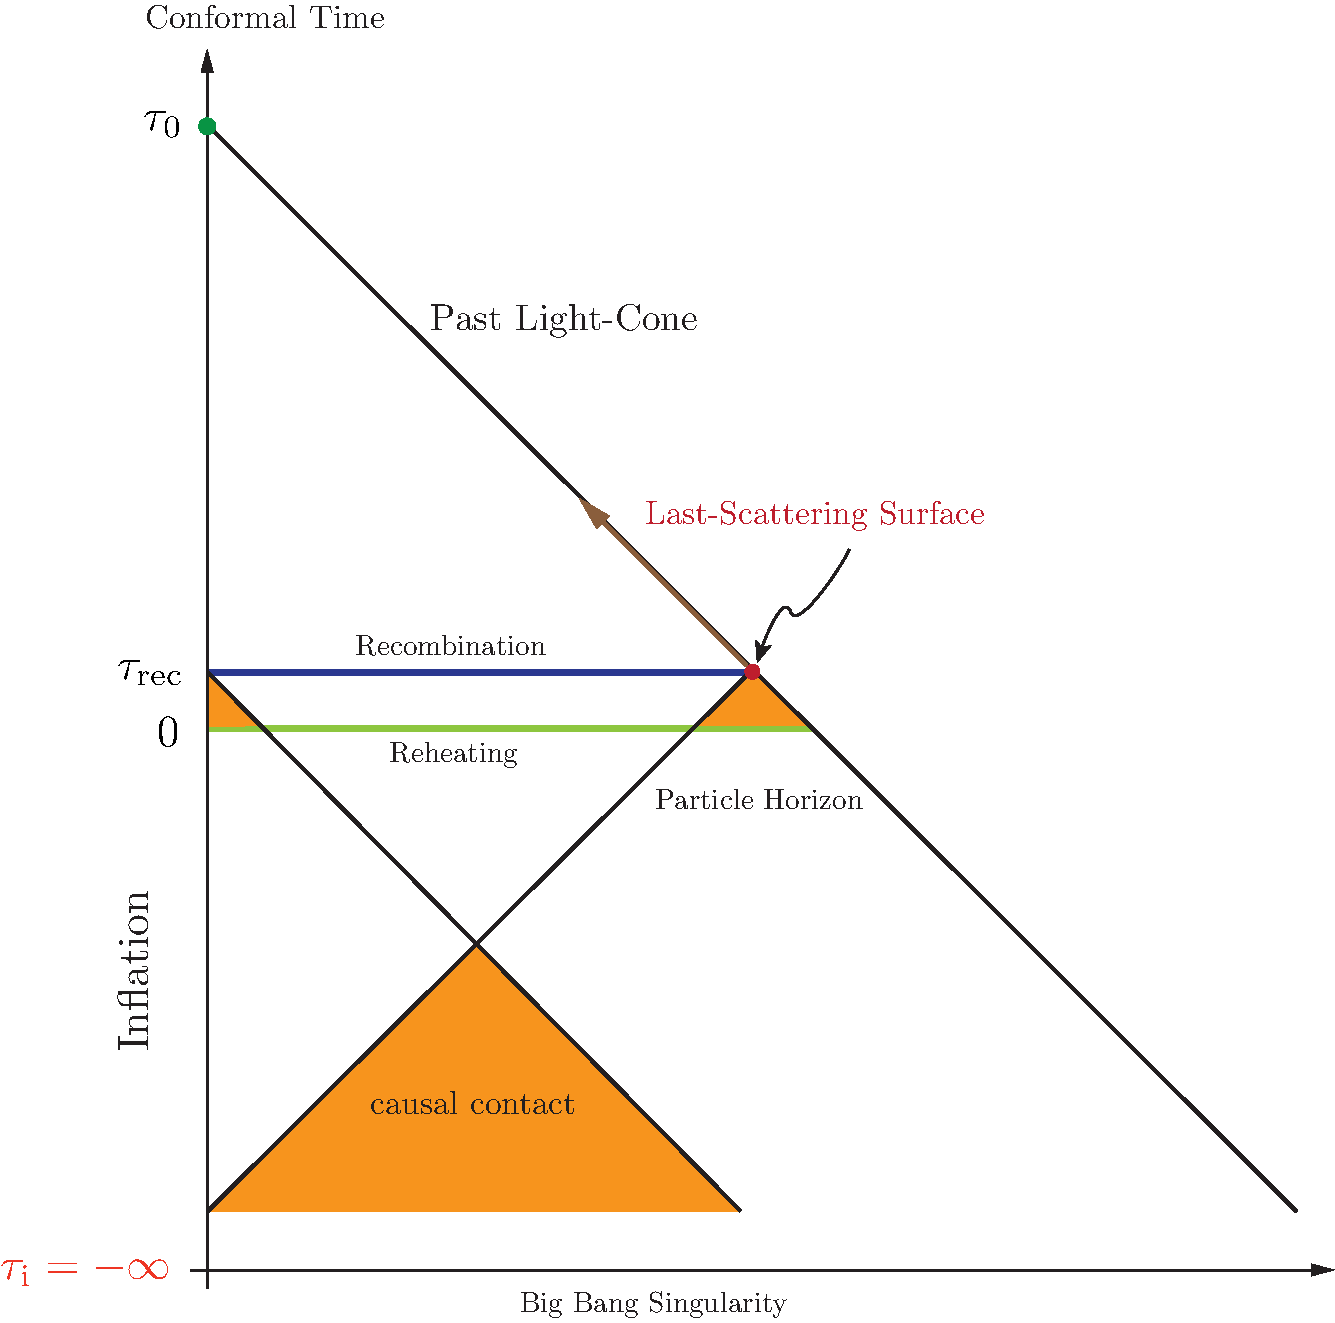
\includegraphics[width=0.95\textwidth]{InflationHorizon}
\caption{インフレーション宇宙論の共形図．インフレーションは共形時間を負の値へと拡張する！ インフレーションの終了は，$\tau = 0$に「見かけの」ビッグバンを作り出す．しかし$\tau =0$に特異点はなく，インフレーションが少なくとも60 $e$-fold続けば，光円錐はより早い時刻で交わる．}
		\label{fig:Conformal2}
\end{figure}

インフレーションを可視化するうえで，共形時空図は実に示唆に富む方法である．
\S\ref{sec:FRW}から，共形時間$\d \tau =\d t/a(t)$で表した平坦なFRW計量を思い出そう．
\beq
\d s^2 =a^2(\tau) \left[- \d \tau^2 + \d {\bf x}^2 \right]\, .
\eeq
また共形座標では，ヌル測地線（$\d s^2$\,=\,$0$）は常に$45^\circ$の角度をなし，$\d \tau = \pm \sqrt{\d {\bf x}^2} \equiv \pm \d r$であることも思い出そう．光は時空の因果構造を決めるので，これはインフレーション宇宙論における地平線を調べるのに適した方法を与える．%and thermal equilibrium

物質優勢期または放射優勢期には，スケール因子は次のように進化する．
\beq
a(\tau) \propto
\left\{ 
\begin{array}{ll}
\tau \quad \,\, \text{RD}\\
\tau^2 \quad \text{MD}
\end{array} \right. \, .
\eeq 
宇宙が常に物質か放射に支配されていた場合に限り，これは$\tau_{\rm i} = 0$に{\it ビッグバン特異点}が存在することを意味する．
\beq
a(\tau_{\rm i} \equiv 0) = 0\, .
\eeq
標準ビッグバン宇宙論に対応する共形図を，図~\ref{fig:Conformal1b}に示す．地平線問題は明らかである．共形図の各時空点には，その因果的な過去を定める過去光円錐が対応する．ある$\tau = \text{一定}$の面上の2点は，その過去光円錐がビッグバン$\tau_{\rm i} = 0$で交われば，因果的に接触している．これは，最終散乱面（$\tau_{\rm CMB}$）が，熱平衡になりえない，因果的につながっていない多数の領域からなっていたことを意味する．したがって，大きなスケールにおけるCMBの一様性は深刻な謎となる．

インフレーション中（$H \approx {\rm const.}$），スケール因子は
\beq
\label{equ:dS}
a(\tau) = -\frac{1}{H \tau}\, ,
\eeq
となり，特異点$a=0$は無限の過去$\tau_{\rm i} \to -\infty$へ押しやられる．
スケール因子(\ref{equ:dS})は，$\tau = 0$で無限大になる！ これは$H = \text{const.}$であるド・ジッター空間を仮定したためであり，インフレーションが永遠に続き，$\tau = 0$が無限の未来$t \to +\infty$に対応することを意味する．実際にはインフレーションはある有限の時刻に終わり，近似(\ref{equ:dS})は初期には有効であっても，インフレーションの終わり近くで成り立たなくなる．したがって面$\tau =0$はビッグバンではなく，インフレーションの終わりである．初期特異点は，共形時間で任意に遠い過去$\tau \ll 0$に押し戻され，光円錐は見かけのビッグバンを通り抜けて延びることができるため，一見つながっていないように見える点も因果的に接触する．
言い換えれば，インフレーションによって「再結合以前には，私たちが考えていたより多くの（共形）時間があった」のである．
これを図~\ref{fig:Conformal2}の共形図にまとめている．



\sectionlink{インフレーションの物理}
\label{sec:SR:source-duplicate-1}

インフレーションは，非常になじみのない物理現象である．
1秒にも満たない間に，宇宙は加速しながら指数関数的に大きくなった．
アインシュタイン重力では，これは負の圧力を持つ源，あるいは同じことだが，ほぼ一定のエネルギー{\rm 密度}を必要とする．
本節では，これが実現される物理的条件を述べる．


\subsectionlink{スカラー場の力学}

\begin{figure}[htbp]
    \centering
        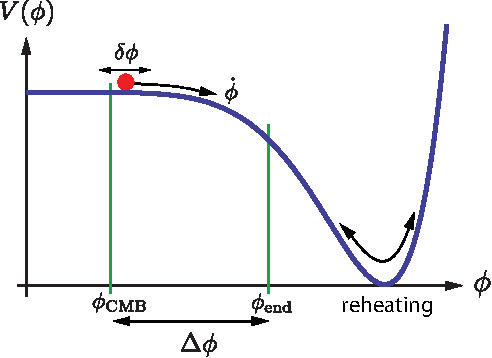
\includegraphics[width=0.45\textwidth]{SmallField}
   \caption{\small インフラトン・ポテンシャルの例．場のポテンシャルエネルギー$V(\phi)$が運動エネルギー$\frac{1}{2} \dot \phi^2$を支配すると，加速が生じる．
運動エネルギーが増大してポテンシャルエネルギーと同程度，$\frac{1}{2} \dot \phi^2 \approx V$になると，$\phi_{\rm end}$でインフレーションは終わる．
CMBの揺らぎは，インフレーション終了の約60 $e$-fold前に，量子揺らぎ$\delta \phi$によって作られる．再加熱の際に，インフラトンのエネルギー密度は放射へと変換される．}
    \label{fig:small}
\end{figure}

最も単純なインフレーション模型は，{\it インフラトン}と呼ばれる単一のスカラー場$\phi$を含む．
ここでは場$\phi$の物理的な正体を特定せず，インフレーションのエネルギー密度の時間発展をパラメータ化する，秩序変数（または時計）として用いるだけにする．
重力に（最小）結合したスカラー場の力学は，次の作用に従う．
\beq
\label{equ:phiaction}
\fbox{$\displaystyle
S = \int \d^4 x \sqrt{-g} \left[\frac{1}{2} R + {1\over 2} g^{\mu \nu} \partial_\mu\phi \, \partial_\nu\phi
-V(\phi) \right]$} = S_{\rm EH} + S_\phi\, .
\eeq
作用(\ref{equ:phiaction})は，重力のアインシュタイン・ヒルベルト作用$S_{\rm EH}$と，正準運動項を持つスカラー場の作用$S_\phi$の和である．
ポテンシャル$V(\phi)$は，スカラー場の自己相互作用を記述する．
スカラー場のエネルギー運動量テンソルは，%given by
\beq
T_{\mu\nu}^{(\phi)} \equiv -\frac{2}{\sqrt{-g}} \frac{\delta S_\phi}{\delta g^{\mu \nu}} = \partial_\mu\phi\partial_\nu\phi-g_{\mu\nu}
\left({1\over 2}\partial^\sigma\phi\partial_\sigma\phi
+V(\phi)\right).
\label{Tscalarfield}
\eeq
である．場の運動方程式は
\beq
\frac{\delta S_\phi}{\delta \phi} = \frac{1}{\sqrt{-g}} \partial_\mu (\sqrt{-g} \partial^\mu \phi) + V_{, \phi}= 0\, ,
\eeq
であり，$V_{, \phi} = \frac{dV}{d\phi}$である．
$g_{\mu \nu}$にFRW計量(\ref{equ:FRW})を仮定し，一様な場$\phi(t, {\bf x}) \equiv \phi(t)$の場合に限ると，スカラー場のエネルギー運動量テンソルは，次の密度と圧力を持つ完全流体(\ref{equ:pf})の形になる．
\begin{eqnarray}
\rho_\phi &=& {1\over 2}\dot\phi^2+V(\phi)\, , \\
p_\phi &=& {1\over 2}\dot\phi^2-V(\phi)\, .
\end{eqnarray}
この結果得られる状態方程式
\beq
\fbox{$\displaystyle
w_\phi  \equiv \frac{p_\phi}{\rho_\phi} = \frac{\frac{1}{2} \dot{\phi}^2 -V}{\frac{1}{2} \dot{\phi}^2 +V}$}\, ,
\eeq
から，ポテンシャルエネルギー$V$が運動エネルギー$\frac{1}{2} \dot{\phi}^2$を支配すると，スカラー場は負の圧力（$w_\phi< 0$）と加速膨張（$w_\phi<-1/3$）をもたらしうることが分かる．
（一様な）スカラー場とFRW幾何の力学は，次の式で決まる．
\beq
\ddot\phi+3H\dot \phi+V_{,\phi}=0 \qquad \text{および} \qquad H^2={1\over 3}\left({1\over 2}\dot\phi^2+V(\phi)\right)\, .
\eeq
ポテンシャルの値が大きいと，場には$H \dot \phi$の項から大きなハッブル摩擦が働く．

\subsectionlink{スローロール・インフレーション}
\label{sec:SR}

一様なスカラー場が支配する宇宙の加速度方程式は，次のように書ける．
\beq
\frac{\ddot a}{a} = - \frac{1}{6} (\rho_\phi + 3 p_\phi) = H^2 (1-\varepsilon)\, ,
\eeq
ここで，
\beq
\varepsilon \equiv \frac{3}{2} (w_\phi + 1) = \frac{1}{2} \frac{\dot \phi^2}{H^2}\, .
\eeq
である．いわゆる{\it スローロール・パラメータ}$\varepsilon$は，ハッブル・パラメータの進化に関係付けられる．
\beq
\fbox{$\displaystyle
\varepsilon = - \frac{\dot H}{H^2}$} = - \frac{d \ln H}{d N}\, ,
\eeq
ここで$\d N = H \d t$である．
$\varepsilon < 1$なら加速膨張が生じる．ド・ジッター極限$p_\phi \to - \rho_\phi$は，$\varepsilon \to 0$に対応する．
この場合，ポテンシャルエネルギーが運動エネルギーを支配する．
\beq
\dot \phi^2 \ll V(\phi)\, .
\eeq
%Inflation occurs if the field is evolving slow enough that the potential energy dominates the kinetic energy, and the second time derivative of $\phi$ is small enough to allow this slow-roll condition to be maintained for a sufficient period. Thus, inflation requires
%\begin{eqnarray}
%\dot{\phi}^2 &\ll& V(\phi)\, \\
%|\ddot{\phi}| &\ll& |3H \dot{\phi}|, |V_{,\phi}|\, .
%\end{eqnarray}
加速膨張が十分に長い時間続くためには，$\phi$の時間に関する2階微分が十分に小さくなければならない．
\beq
|\ddot{\phi}| \ \ll \ |3H \dot{\phi}|\, , \, |V_{,\phi}|\, .
\eeq
これは，第2のスローロール・パラメータが小さいことを必要とする．
\beq
\eta = - \frac{\ddot \phi}{H \dot \phi} = \varepsilon - \frac{1}{2 \varepsilon} \frac{d \varepsilon}{d N}\, ,
\eeq
ここで$|\eta| < 1$は，1 $e$-fold当たりの$\varepsilon$の相対変化が小さいことを保証する．
%Satisfying these conditions requires the smallness of two dimensionless quantities known as {\it slow-roll parameters}
スローロール条件$\varepsilon, |\eta| < 1$は，インフレーション・ポテンシャルの形に対する条件として表すこともできる．
\begin{equation}
\fbox{$\displaystyle \epsilon_{\rm v}(\phi) \equiv \frac{M_{\rm pl}^2}{2} \left(\frac{V_{,\phi}}{V}\right)^2 $}\, ,
\end{equation}
および
\begin{equation}
\fbox{$\displaystyle
\eta_{\rm v}(\phi) \equiv M_{\rm pl}^2 \frac{V_{,\phi\phi}}{V} $}\, .
\end{equation}
ここでは$\epsilon_{\rm v}$と$\eta_{\rm v}$が無次元であることを明示するため，一時的にプランク質量を再導入した．
以下では再び$M_{\rm pl}$を1と置く．
スローロール領域
\beq
\label{equ:SR}
\epsilon_{\rm v}, |\eta_{\rm v}| \ll 1\, ,
\eeq
では，背景の進化は
\begin{eqnarray}
H^2 &\approx& {1\over 3} V(\phi) \approx \text{const.}\, , \label{equ:SRH}\\
\dot{\phi} &\approx& -\frac{V_{,\phi}}{3H} \label{equ:SRphi}\, ,
\end{eqnarray}
となり，時空は近似的に{\it ド・ジッター}時空となる．
\begin{equation}
a(t) \sim e^{Ht}\, . % , \quad  {\rm where} \quad H \approx \text{const}\, .
\end{equation}
パラメータ$\epsilon_{\rm v}$と$\eta_{\rm v}$は，{\it ハッブル・スローロール・パラメータ}$\varepsilon$および$\eta$と区別するため，{\it ポテンシャル・スローロール・パラメータ}と呼ばれる．
スローロール近似では，ハッブルおよびポテンシャルのスローロール・パラメータは次のように関係する（付録~\ref{sec:HSR}参照）．
\beq
\varepsilon \approx \epsilon_{\rm v} \, , \qquad \eta \approx \eta_{\rm v} - \epsilon_{\rm v}\, .
\eeq
%To understand the relation between the slow-roll condition (\ref{equ:SR}) and inflation it is helpful to convince yourself that the following is true
%\beq
%\label{equ:SR2}
%\frac{\ddot{a}}{a} = H^2 \left(1+\frac{\dot H}{H^2}\right) \approx H^2 (1-\epsilon_{\rm v})\, .
%\eeq
%Consequently, if the slow-roll approximation is valid ($\epsilon_{\rm v} \ll 1$), then inflation is guaranteed. However, this condition is sufficient but not necessary since the validity of the slow-roll approximation was required to establish the second equality in (\ref{equ:SR2}).

スローロール条件が破れると，インフレーションは終了する．%(\ref{equ:SR})
%\footnote{This can be made exact by the use of Hubble slow-roll parameters instead of the potential slow-roll parameters we introduced here (see Appendix B).}
\beq
\varepsilon(\phi_{\rm end}) \equiv 1\, , \qquad \epsilon_{\rm v}(\phi_{\rm end}) \approx 1\, .
\eeq
インフレーションが終了するまでの$e$-fold数は，
\begin{eqnarray}
N(\phi) &\equiv& \ln \frac{a_{\rm end}}{a} \nonumber\\
&=&\int_t^{t_{\rm end}} H \d t = \int_\phi^{\phi_{\rm end}} \frac{H}{\dot \phi} \d \phi 
\approx \int_{\phi_{\rm end}}^\phi \frac{V}{V_{,\phi}} \d \phi \, , \label{equ:Nphi}
\end{eqnarray}
である．ここでは，スローロールの結果(\ref{equ:SRH})と(\ref{equ:SRphi})を用いた．
結果(\ref{equ:Nphi})は，次のようにも書ける．
\beq
\fbox{$\displaystyle
N(\phi) = \int_{\phi_{\rm end}}^\phi \frac{\d \phi}{\sqrt{2\varepsilon}}  \approx \int_{\phi_{\rm end}}^\phi \frac{\d \phi}{\sqrt{2\epsilon_{\rm v}}} $}\, .
\eeq
地平線問題と平坦性問題を解くには，インフレーションの総$e$-fold数が約60を超える必要がある．
\beq
N_{\rm tot} \equiv \ln \frac{a_{\rm end}}{a_{\rm start}} \gtrsim 60\, .
\eeq
正確な値は，インフレーションのエネルギースケールと，インフレーション後の再加熱の詳細に依存する．
CMBで観測される揺らぎは，インフレーションの終了より$N_{\rm cmb} \approx 40-60$ $e$-fold前に作られる（正確な値は，やはり再加熱とインフレーション後の宇宙の熱史の詳細に依存する）．以下の積分制約から，それに対応する場の値$\phi_{\rm cmb}$が得られる．
\beq
 \int_{\phi_{\rm end}}^{\phi_{\rm cmb}} \frac{\d \phi}{\sqrt{2\epsilon_{\rm v}}} = N_{\rm cmb} \approx 40 -60\, .
\eeq


\subsectionlink{具体例：$m^2 \phi^2$インフレーション}

一例として，おそらく最も単純なインフレーション模型，すなわち質量項によって駆動される単一場インフレーションのスローロール解析を行おう．
\beq
V(\phi) = \frac{1}{2} m^2 \phi^2\, .
\eeq
スローロール・パラメータは，
\beq
\epsilon_{\rm v}(\phi) = \eta_{\rm v}(\phi) = 2 \left( \frac{M_{\rm pl}}{\phi}\right)^2\, .
\eeq
である．スローロール条件$\epsilon_{\rm v}, |\eta_{\rm v}| < 1$を満たすには，インフラトンについて，プランク質量を超える場の値を考えなければならない．
\beq
\phi > \sqrt{2} M_{\rm pl} \equiv \phi_{\rm end}\, .
\eeq
インフラトンの場の値と，インフレーション終了までの$e$-fold数の関係は，
\beq
N(\phi) = \frac{\phi^2}{4 M_{\rm pl}^2} - \frac{1}{2}\, .
\eeq
である．CMBで観測される揺らぎは，次の場の値で生成される．
\beq
\phi_{\rm cmb} = 2 \sqrt{N_{\rm cmb}} \, M_{\rm pl} \sim 15 M_{\rm pl}\, .
\eeq
次の講義では，$m^2 \phi^2$インフレーションが生成する揺らぎのスペクトルを計算する際に，この例に戻る．

\begin{thm}[$m^2 \phi^2$インフレーション]
$m^2 \phi^2$インフレーションについて，上記のスローロールの結果を確かめよ．
\label{ex:chaotic}
\end{thm}

\subsectionlink{再加熱}

インフレーションが終了すると，スカラー場はポテンシャルの極小点のまわりで振動し始める．
このコヒーレントな振動の時期には，スカラー場は圧力のない物質のように振る舞う．
\beq
\label{equ:coherent}
\frac{d \bar \rho_\phi}{dt} + 3H \bar \rho_\phi = 0\, .
\eeq

\begin{thm}[スカラー場のコヒーレントな振動]
$\phi$の運動方程式から，式~(\ref{equ:coherent})を確かめよ．
\label{ex:coherent}
\end{thm}

インフラトン場と他の粒子との結合によって，インフラトンのエネルギーが崩壊する．
\beq
\frac{d \bar \rho_\phi}{dt} +(3H+ \Gamma_\phi) \bar \rho_\phi = 0\, .
\eeq
結合パラメータ$\Gamma_\phi$は，複雑で模型に依存した物理過程によって決まるが，ここではそれらを概説する時間はない．
最終的にインフレーションのエネルギー密度は標準模型の自由度へと変換され，熱いビッグバンが始まる．
%a few words on preheating

再加熱は豊かで複雑な主題であり，本講義では十分に扱うことができない．
詳しく知りたい読者には，Bassettらの総説\cite{BassettReview}を勧める．


%Give expression for number of e-folds.


\subsectionlink{インフレーションの模型}

インフレーションの根本的な微視的起源は，今も謎である．インフラトンとは何か，インフレーション・ポテンシャルはどのような形か，なぜ宇宙は高エネルギー状態から始まったのか，といった基本的な問いは未解決のままである．インフレーションの物理を説明するという課題は，非常に難しい．インフレーションは，地上の粒子加速器では到底到達できない，巨大なエネルギースケール（$\sim 10^{15}$ GeVにも達するかもしれない）で起こったと考えられている．したがって，インフレーション期を記述するには，既知の物理法則を大幅に外挿する必要があり，最近までは，インフレーションの力学を現象論的にパラメータ化することしかできなかった．\footnote{最近では，インフレーションの系統的な有効場の理論による記述\cite{PaoloEFT, WeinbergEFT}と，弦理論からのトップダウンによるインフレーション・ポテンシャルの導出\cite{BMReview}の両方で進展があった．}このアプローチでは，適切なインフレーション・ポテンシャル関数$V(\phi)$を仮定し（よく使われる二つの例については図~\ref{fig:small}と図~\ref{fig:large}を参照），そこから実験的予言を計算する．次の講義で見るように，原始揺らぎのスペクトルの詳細は，インフラトン・ポテンシャルの正確な形に依存する．


\subsubsection{単一場スローロール・インフレーション}

インフレーション模型を定義することは，インフラトンの作用（ポテンシャル項と運動項）およびその重力との結合を指定することに等しい．
これまでは，最も単純な模型，すなわち次の作用で特徴付けられる単一場スローロール・インフレーションの言葉で議論してきた．
\beq
\label{equ:simple}
S = \int \d^4 x \sqrt{-g} \left[\frac{1}{2} R + {1\over 2} g^{\mu \nu} \partial_\mu\phi \, \partial_\nu\phi
-V(\phi) \right]\, .
\eeq
CMBの揺らぎが生成された$\phi_{\rm cmb}$の時点（{\bf 第2講}参照）から，$\phi_{\rm end}$でインフレーションが終わるまでのインフラトン場の力学は，インフレーション・ポテンシャル$V(\phi)$の形によって決まる．
$V(\phi)$のさまざまな可能性は，インフラトン場が移動する距離$\Delta \phi \equiv \phi_{\rm cmb} -\phi_{\rm end}$が，プランク単位で測って大きいか小さいかによって分類すると便利である．

\begin{figure}[htbp]
    \centering
        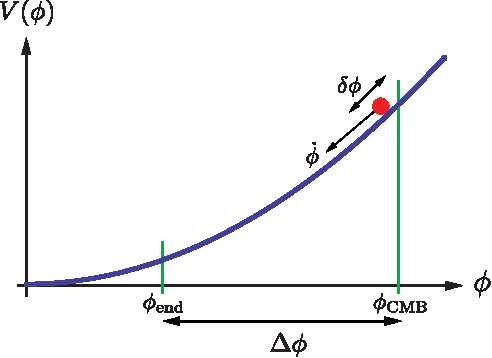
\includegraphics[width=0.4\textwidth]{LargeField}
   \caption{\small 大場インフレーション．重要な一群のインフレーション模型では，インフレーションの力学はポテンシャルの単一の単項式項$V(\phi) \propto \phi^p$によって駆動される．これらの模型では，インフラトン場はインフレーション中にプランク質量を超える範囲$\Delta \phi > M_{\rm pl}$を動き，量子力学的揺らぎによって大振幅の重力波が生成される（{\bf 第2講}参照）．}
    \label{fig:large}
\end{figure}

\begin{enumerate}
\item {\it 小場インフレーション}

小場模型では，場は小さな（プランク質量未満の）距離$\Delta \phi < M_{\rm pl}$を動く．
これは将来の観測に関係する．小場模型は，インフレーション中に生成される重力波の振幅が小さすぎて検出できないと予言するからである（{\bf 第2講}参照）．
このような小場の進化を生むポテンシャルは，しばしば{\it 自発的対称性の破れ}の機構で現れる．この場合，場は不安定な平衡点から離れて，ずれた位置にある真空に向かって転がる（図~\ref{fig:small}参照）．簡単な例は，ヒッグス型ポテンシャルである．
\beq
V(\phi) = V_0 \left[ 1- \left(\frac{\phi}{\mu}\right)^2 \right]^2\, .
\eeq
より一般に，小場模型は局所的に次の展開で近似できる．
\beq
V(\phi) = V_0 \left[ 1 - \left(\frac{\phi}{\mu}\right)^p\right] + \cdots \ ,
\eeq
ここで省略記号は，インフレーションの終わり近くや再加熱中に重要となる高次の項を表す．

歴史的に有名なインフレーション・ポテンシャルが，{\it コールマン・ワインバーグ・ポテンシャル}である\cite{Linde:1981mu, Albrecht:1982wi}．
\beq
V(\phi) = V_0 \left[ \left(\frac{\phi}{\mu}\right)^4 \left( \ln \left( \frac{\phi}{\mu}\right) - \frac{1}{4}\right) + \frac{1}{4}\right]\, ,
\eeq
これは，電弱理論や大統一理論で，輻射補正によって誘起される対称性の破れのポテンシャルとして現れる．
$SU(5)$理論に基づく当初のパラメータ$V_0$と$\mu$の値は，インフレーション揺らぎの小さな振幅とは両立しないものの，コールマン・ワインバーグ・ポテンシャルは今もよく使われる現象論的模型である（例えば\cite{Shafi:2006cs}参照）．

\item {\it 大場インフレーション}

大場模型では，インフラトン場は大きな場の値から始まり，原点$\phi=0$にある極小点へと進化する．場の変化がプランク質量を超える場合，$\Delta \phi > M_{\rm pl}$には，インフレーションが生み出す重力波は近い将来に観測されるはずである．

典型的な大場模型は，単一の単項式項がポテンシャルを支配する{\it カオティック・インフレーション}である（図~\ref{fig:large}参照）．
\beq
V(\phi) = \lambda_p \phi^p\, .
\eeq
このようなポテンシャルでは，プランク質量を超える場の値$\phi \gg M_{\rm pl}$に対して，スローロール・パラメータは小さくなる（スローロール条件が結合定数$\lambda_p$に依存しないことに注意しよう）．ただし，密度揺らぎの振幅を小さくするには（{\bf 第2講}参照），インフラトンの自己結合が非常に小さく，$\lambda_p \ll 1$でなければならない．この条件は，ポテンシャルエネルギー（密度）がプランク・スケール未満，$V \ll M_{\rm pl}^4$であることを自動的に保証し，量子重力効果は必ずしも重要ではない（ただし{\bf 第5講}の\S\ref{sec:UV}を参照）．

最も美しいインフレーション模型の一つが，ポテンシャルが次の形を取る{\it ナチュラル・インフレーション}である（図~\ref{fig:natural}参照）．
\beq 
V(\phi)
= V_0 \left[ \cos \left(\frac{\phi}{ f}\right) + 1\right]\, . 
\eeq
このポテンシャルは，インフラトン場をアクシオンとしたときにしばしば現れる．
パラメータ$f$によって，模型は小場型にも大場型にもなりうる．
しかし，大きな場の変化$2\pi f > M_{\rm pl}$に対してナチュラル・インフレーションを考えることは，特に魅力的である．アクシオンではシフト対称性を利用して，場の範囲が大きくても，ポテンシャルを補正項から保護できるからである（\S\ref{sec:UV}参照）．

\begin{figure}[htbp]
    \centering
        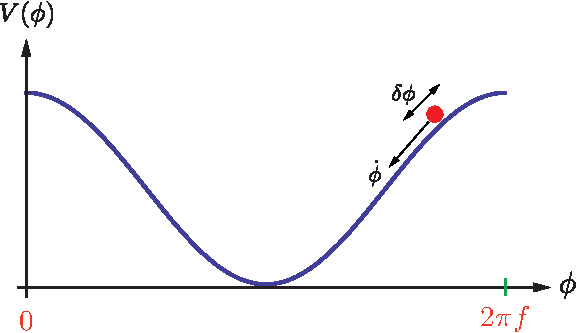
\includegraphics[width=0.5\textwidth]{NaturalInflation}
   \caption{\small ナチュラル・インフレーション．周期$2\pi f$がプランク質量を超える場合，この模型は大きな重力波振幅を自然に実現できる．}
    \label{fig:natural}
\end{figure}

\end{enumerate}
%\subsectionlink{Initial Conditions and Inflationary Attractors}

%\subsubsection{The Overshoot Problem}

%phase space

%\subsubsection{The Patch Problem}

%relation to event horizon


\subsubsection{単一場スローロールを超えて}


インフレーション膨張を得るための可能性は，（いら立たしいほどに）多様である．
インフレーションは一つのパラダイム，初期宇宙の理論の枠組みであるが，一意な理論ではない．
異なる理論的動機と観測的予言を持つ，多数の現象論的模型が提案されている．
本講義の大部分では，今述べた最も単純な単一場スローロール模型に焦点を当てる．
しかし，この短い節では，インフレーションの模型構築のより広い全体像に触れないという罪を，少しでも免れたい（文献\cite{LythRiotto}も参照）．

最も単純なインフレーションの作用(\ref{equ:simple})は，いくつかの明白な方法で拡張できる．

\begin{enumerate}
\item {\it 重力との非最小結合．}

作用(\ref{equ:simple})は，インフラトン場と計量の直接的な結合がないという意味で，最小結合と呼ばれる．原理的には，インフラトンと重力子の間の非最小結合を考えてもよい．しかし実際には，非最小結合理論は，場の再定義によって最小結合理論として書ける．

\item {\it 修正重力．}

同様に，作用のアインシュタイン・ヒルベルト部分が高エネルギーで修正される可能性も考えられる．しかし，このような重力の紫外での修正の最も単純な例である，いわゆる$f(R)$理論も，ポテンシャル$V(\phi)$を持つ最小結合スカラー場へと変換できる．

\item {\it 非正準運動項．}

作用(\ref{equ:simple})は，正準運動項を持つ．
\beq
{\cal L}_\phi = X - V(\phi)\, , \qquad X \equiv \frac{1}{2} g^{\mu \nu} \partial_\mu \phi \partial_\nu \phi\, .
\eeq
この場合，インフレーションは，ポテンシャル$V(\phi)$が非常に平坦なときにしか起こらない．
しかし，より一般には，高エネルギーの理論に，非正準運動項を持つ場が含まれることを考えられる．
\beq
\label{equ:kin}
{\cal L}_\phi = F(\phi, X) - V(\phi)\, , 
\eeq
ここで$F(\phi,X)$は，インフラトン場とその微分の何らかの関数である．
(\ref{equ:kin})のような作用では，インフレーションが運動項によって駆動され，急なポテンシャルがあっても起こりうる．

\item {\it 複数の場．}

インフレーション中に複数の場が力学的に重要であることを許すと，インフレーションの力学（および揺らぎの生成機構）の可能性は飛躍的に広がり，理論はその予言能力の多くを失う．
多場インフレーション模型の数多くの可能性の一部は，文献\cite{WandsMulti}で概説されている．
\end{enumerate}


%\subsubsection{Multi-Field Inflation} 


%hybrid inflation

%\subsubsection{Non-Trival Kinetic Terms}

%DBI inflation


\newpage
\sectionlink{{\sl まとめ}：第1講}

\vskip 10pt
通常のFRW宇宙論の初期条件は，高度に微調整されているように見える．
地平線問題も平坦性問題も，標準ビッグバンの進化の間，共動ハッブル半径$(aH)^{-1}$が時間とともに単調に増大するという事実に起因する．
一方，インフレーション中には共動ハッブル半径が一時的に減少する．
\begin{figure}[h!]
	\centering
		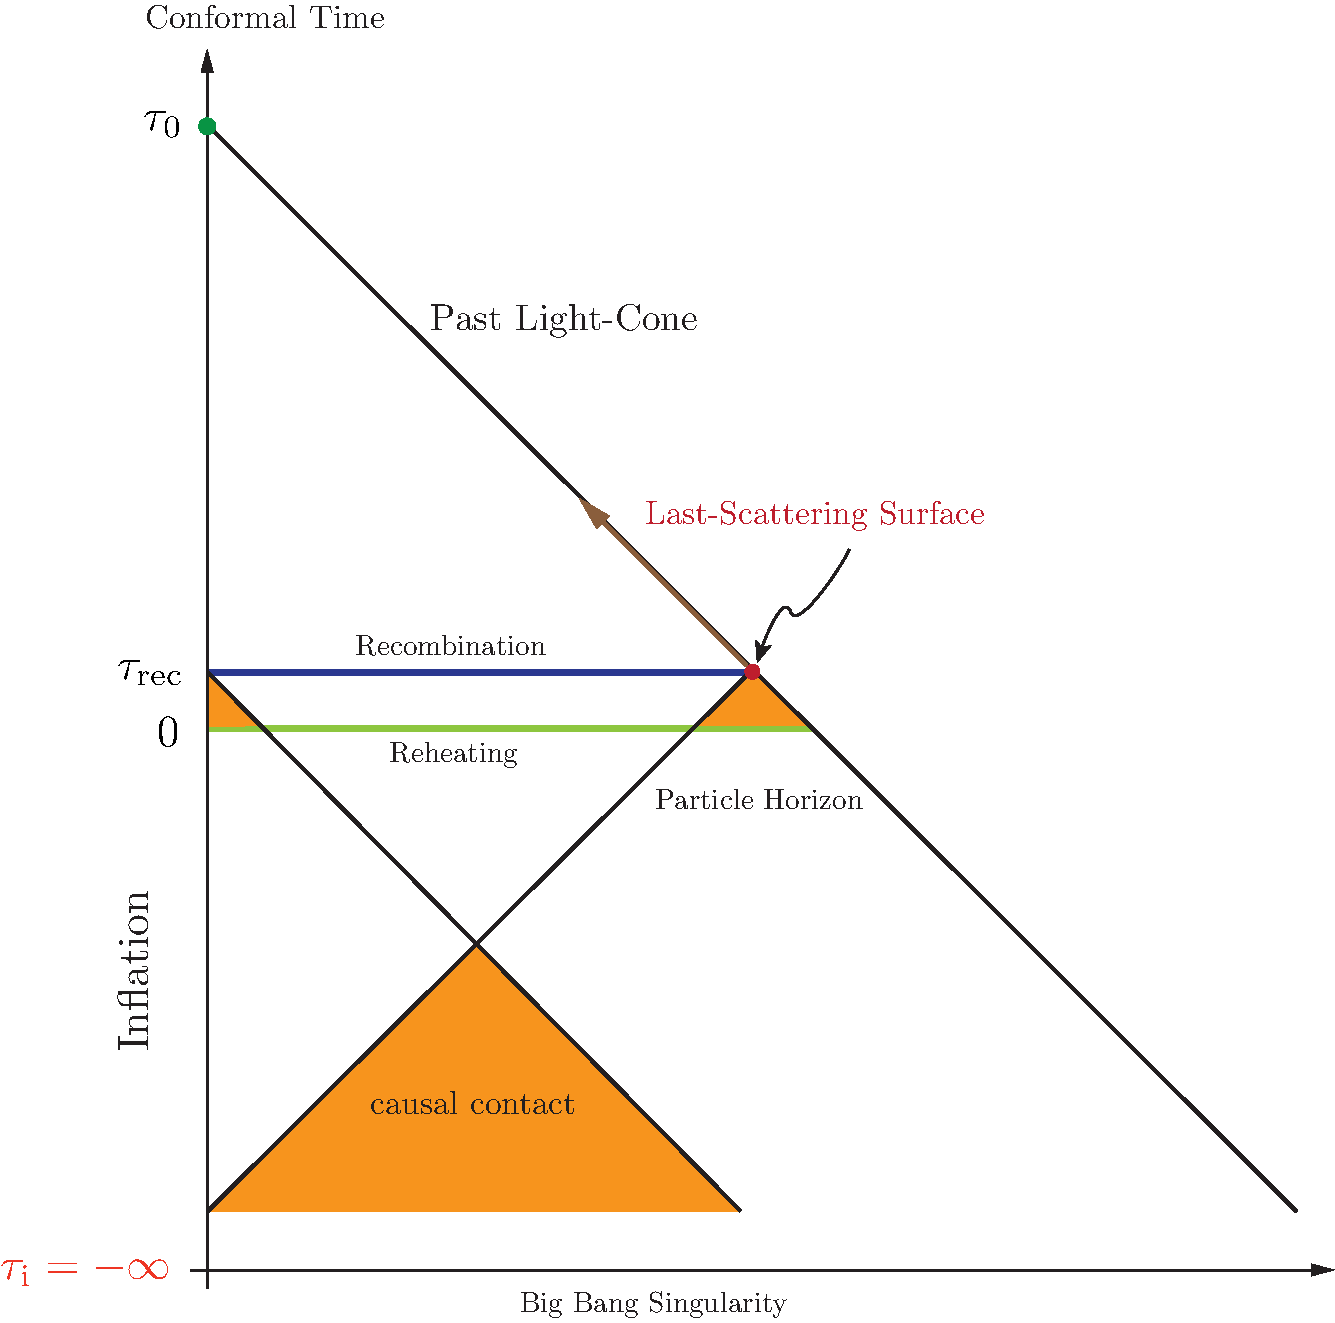
\includegraphics[width=0.55\textwidth]{InflationHorizon}
\caption{インフレーション宇宙論の共形図．インフレーションは共形時間を負の値へと拡張する！ インフレーションの終了は，$\tau = 0$に「見かけの」ビッグバンを作り出す．しかし$\tau =0$に特異点はなく，インフレーションが少なくとも60 $e$-fold続けば，光円錐はより早い時刻で交わる．}
		\label{fig:Conformal3}
\end{figure}
これによって初期宇宙の因果構造が変わり，地平線問題は，通常のFRW膨張を任意に早い時刻まで外挿することによって生じた見かけの問題となる．
アインシュタイン方程式から，ハッブル半径の縮小は加速膨張に対応し，それが負の圧力を持つ成分で宇宙が満たされている場合に生じることを示せる．
したがって，インフレーションの三つの同値な条件は，
\beq
\frac{d (aH)^{-1}}{dt}\ < \ 0 \qquad \Rightarrow \qquad \frac{d^2 a}{d t^2} \ > \ 0 \qquad \Rightarrow \qquad p\ < \ - \frac{\rho}{3} \ \ . \nonumber
\eeq
である．負の圧力を持つ流体は，次の作用を持つスカラー場$\phi$，すなわちインフラトンによって模型化できる．
\beq
S = \int \d^4 x \sqrt{-g} \left[ \frac{1}{2}R + \frac{1}{2} g^{\mu \nu} \partial_\mu \phi \partial_\nu \phi - V(\phi) \right]\, . \nonumber
\eeq
スローロール条件が満たされれば，これはインフレーションを引き起こす．
\beq
\epsilon_{\rm v} = \frac{\Mp^2}{2} \left(\frac{V_{, \phi}}{V} \right)^2\, , \qquad \eta_{\rm v} = \Mp^2 \frac{V_{, \phi \phi}}{V}\, , \qquad \quad \epsilon_{\rm v}, |\eta_{\rm v}| < 1\, . \nonumber
\eeq
このとき，インフレーションによる膨張の$e$-fold数は，
\beq
N(\phi) = \int_{\rm \phi_{\rm end}}^\phi \frac{\d \phi}{\sqrt{2 \epsilon_{\rm v}}}\, .
\eeq
である．地平線問題を解くには，総$e$-fold数が少なくとも60必要である．
CMBの揺らぎは，インフレーション終了の約60 $e$-fold前に，4 $e$-foldの間に生成される．
上記の作用で記述される単一場スローロール・インフレーションという限られた枠組みの中でも，インフレーション・ポテンシャル$V(\phi)$の異なる選び方によって特徴付けられる，多数のインフレーション模型がある．



\sectionlink{{\sl 問題集}：第1講}

\vskip 10pt
\begin{thmP}[一様かつ等方的な空間]\label{pro:FRW}
一様かつ等方的な空間は，並進不変性と回転不変性によって特徴付けられる．
3次元では，単純な位相を持つ一様かつ等方的な空間は，次の3種類しか存在しないことを確認せよ．
\begin{enumerate}
\item[i)] 平坦な空間
\item[ii)] 正の一定曲率を持つ3次元球面
\item[iii)] 負の一定曲率を持つ3次元双曲空間．
\end{enumerate}
2次元の類例の方が，視覚的に捉えやすい．
3次元ユークリッド空間への2次元球面の埋め込みを考えよう．
\beq
x^2 + y^2 + z^2 = a^2\, ,
\eeq
ここで$a$は球面の半径である．
球面上の誘導計量が，次のようになることを示せ．
\beq
\d \ell_2^2 = \frac{\d r'^2}{1-(r'^2/a^2)} + r'^2 \d \phi^2\, , 
\eeq
ここで$x=r' \cos \phi$および$y=r' \sin \phi$である．
極限$a^2 \to \infty$は，平坦な空間（平面）に対応する．
負の$a^2$は，負の一定曲率を持つ空間に対応する．
これは3次元ユークリッド空間に埋め込むことはできない．（代わりに，計量$\d \ell_2^2 = \d x^2 + \d y^2 - \d z^2$を持つ空間への，$x^2 + y^2 -z^2 =-a^2$の埋め込みを考えよ．）

動径座標を再スケールすると，計量は次の形にできる．
\beq
\d \ell_2^2 = |a^2| \left(\frac{\d r^2}{1-k r^2} + r^2 \d \phi^2 \right)\, ,
\eeq
ここで，球面（$a^2 > 0$）では$k=+1$，双曲空間（$a^2 < 0$）では$k=-1$，平面（$a^2 =0$）では$k=0$である．

上の議論を，一様かつ等方的な3次元空間の4次元ユークリッド空間への埋め込みに一般化せよ．その計量が次のようになることを示せ．
\beq
\d \ell_3^2 = a^2 \left(\frac{\d r^2}{1-k r^2} + r^2 \d \Omega^2 \right)\, , \qquad \d \Omega^2 \equiv \d \theta^2 + \sin^2 \theta \d \phi^2\, ,
\eeq
あるいは，
\beq
\d \ell_3^2 = a^2 \left[\d \chi^2 +\left( 
\begin{array}{c} \sinh^2 \chi \\ \chi^2 \\ \sin^2 \chi \\
\end{array} \right) \d \Omega^2\right] \quad \begin{array}{l} k=-1 \\ k=0 \\ k=+1 \end{array} \, .
\eeq
空間の一様性と等方性を保つ，時間依存する唯一の4次元時空が，FRW計量であることを確認せよ．
\beq
\d s^2 = \d t^2 - a^2(t)  \left(\frac{\d r^2}{1-k r^2} + r^2 \d \Omega^2 \right)\, .
\eeq
\end{thmP}

\begin{thmP}[共形時間]
共形時間$\tau$を$a$の関数として表す，いくつかの簡単な式を導け．

\begin{enumerate}
\item 物質優勢宇宙では$\tau \propto a^{1/2}$，放射優勢宇宙では$\tau \propto a$となることを示せ．
\item 物質と放射のみを含み，$a_{\rm eq}$で両者が等しくなる宇宙を考えよ．次を示せ．
\beq
\label{equ:taueq}
\tau = \frac{2}{\sqrt{\Omega_m H_0^2}} \left[ \sqrt{a+a_{\rm eq}} - \sqrt{a_{\rm eq}}\right]\, .
\eeq
現在の共形時間はいくらか．脱結合時にはいくらか．
\item 好みのソフトウェア（例えばMathematicaやMaple）を使って，私たちの宇宙（ダークエネルギー，物質，放射で満たされている）の共形時間を数値的に計算せよ．現在と脱結合時の共形時間を求めよ．この結果と，物質・放射のみの宇宙に対する解析的結果である式~(\ref{equ:taueq})の誤差は，何パーセントか．
\end{enumerate}
\end{thmP}

\begin{thmP}[フリードマン方程式]\label{pro:Friedmann}
FRW時空(\ref{equ:FRW})のリッチ・テンソルとリッチ・スカラーを導け．
\beq
R_{00} = -3 \frac{\ddot a}{a}\, , \qquad R_{ij} = \delta_{ij} \left[2 \dot a^2 + a \ddot a + 2\frac{k}{a^2} \right]\, , \qquad R= g^{\mu \nu} R_{\mu \nu} = 6 \left[\frac{\ddot a}{a} + \left(\frac{\dot a}{a}\right)^2 + \frac{k}{a^2}\right]\, .
\eeq
アインシュタイン方程式(\ref{equ:Einstein})の00成分が，フリードマン方程式を与えることを確かめよ．
\beq
\left(\frac{\dot a}{a}\right)^2 =  \frac{8\pi G}{3} \rho - \frac{k}{a^2} \, .
\eeq
アインシュタイン方程式(\ref{equ:Einstein})のトレースが，加速度方程式を与えることを確かめよ．
\beq
\frac{\ddot a}{a} = - \frac{4\pi G}{3} (\rho + 3 p) \, .
\eeq
2本のフリードマン方程式から，連続の式が従うことを示せ．
\beq
\dot \rho = - 3H (\rho + p)\, .
\eeq
次の式から連続の式を導け．
\beq
\label{equ:conservation}
\nabla_\mu T^\mu_{\ \nu} = 0\, .
\eeq
（ヒント：式~(\ref{equ:conservation})を$U^\mu$と縮約し，完全流体のエネルギー運動量テンソルと4元速度の性質を使え．クリストッフェル記号は不要である！）
\end{thmP}

%\begin{thm}[Scalar Fluid]
%From the scalar field action derive the energy-momentum tensor
%\beq
%T_{\mu \nu} =
%\eeq
%Show that in the homogeneous limit, $\phi(t, {\bf x}) \to \phi(t)$ this takes the form of a perfect fluid (x.x) with
%\beq
%\rho = \frac{1}{2}\dot \phi^2 + V(\phi)\, , \qquad p=\frac{1}{2}\dot \phi^2 - V(\phi)\, .
%\eeq
%\end{thm}

%\begin{thm}[Preheating]
%\end{thm}

\begin{thmP}[$\lambda \phi^4$インフレーション]\label{pro:case}
$\lambda \phi^4$インフレーションのスローロール力学を導け．
\end{thmP}


\begin{thmP}[$m \phi^2$インフレーションの位相空間]\label{pro:case2}
Mukhanovの教科書\cite{Mukhanov}で，$m^2 \phi^2$インフレーションのアトラクターとしての振る舞いについて読め．
\end{thmP}


\newpage


